\documentclass[10pt]{article}
\usepackage{tmlr}
\usepackage{hyperref}
\usepackage{url}
\usepackage{booktabs}
\usepackage{graphicx}
\usepackage{tikz}
\usetikzlibrary{arrows.meta, shapes.geometric, positioning, fit, backgrounds, calc, decorations.pathreplacing, matrix, patterns}
\usepackage{pgfplots}
\pgfplotsset{compat=1.18}
\usepackage{float}
\usepackage{xcolor}
\definecolor{nvidiagreen}{RGB}{118,185,0}
\definecolor{nvidiagray}{RGB}{100,100,100}
\definecolor{hopperblue}{RGB}{0,112,192}
\definecolor{blackwellred}{RGB}{192,0,0}
\definecolor{ambercolor}{RGB}{255,165,0}
\definecolor{lightgray}{RGB}{230,230,230}
\definecolor{lightblue}{RGB}{173,216,230}
\definecolor{lightyellow}{RGB}{255,255,200}
\definecolor{lightgreen}{RGB}{200,240,200}


\title{GPU Kernel Optimization for Mixture-of-Experts on Hopper and Blackwell: A Survey}

\author{\name Anonymous Authors \email anon@anon.org \\ \addr Anonymous Institution}

\def\month{MM}\def\year{YYYY}
\def\openreview{\url{https://openreview.net/forum?id=XXXX}}

\begin{document}
\maketitle

\begin{abstract}
Deploying trillion-parameter Mixture-of-Experts (MoE) models at scale is, in practice, a GPU kernel engineering problem. Per-token routing, grouped GEMMs with variable expert loads, and scatter/gather across HBM all conspire to keep effective arithmetic intensity well below the compute ceiling of modern accelerators, turning what would otherwise be straightforward matmul into a sustained memory-bandwidth challenge. The NVIDIA Hopper (H100) and Blackwell (B200/GB200) architectures have sharpened this challenge while simultaneously providing new tools to address it: asynchronous warp-group MMA (WGMMA), the Tensor Memory Accelerator (TMA), thread-block clusters with distributed shared memory, a dedicated Tensor Memory (TMEM), and native FP4/FP8 with microscaling---each of which demands a substantially different programming model than the generation before it.

This survey maps the resulting technical landscape. We trace how high-performance matmul abstractions have evolved from hand-written CUDA through CUTLASS, CuTe/CuTeDSL, Triton, ThunderKittens, and HipKittens, and we use the FlashAttention lineage (FA1--FA4) as a running case study in IO-aware kernel co-design with hardware. Against that backdrop we survey MoE-specific systems---MegaBlocks, ScatterMoE, Tutel, DeepSpeed-MoE, FasterMoE, SonicMoE, DeepGEMM, DeepEP---focusing on grouped GEMM kernel design, distributed all-to-all communication, and the fusion patterns that exploit L2 and SMEM locality between otherwise separate kernel launches. A worked case study of L2-cache-warm megakernel fusion and time-multiplexed SMEM fusion for a SonicMoE-style MoE forward pass makes the cost model concrete. We close with an assessment of cross-vendor portability to AMD CDNA and a discussion of open problems: FP4 training kernels, compute-overlapped all-to-all, compiler automation of megakernel fusion, and heterogeneous-precision MoE.
\end{abstract}

\section{Introduction}
\label{sec:intro}

The scaling of Large Language Models (LLMs) has been the defining trend in machine learning systems over the past five years~\citep{brown2020gpt3,touvron2023llama,achiam2023gpt4}. Dense scaling, however, faces a hard wall: training and serving costs grow super-linearly with parameter count. Mixture-of-Experts (MoE) architectures~\citep{shazeer2017outrageously,fedus2022switch,lepikhin2021gshard,jiang2024mixtral} sidestep this wall by activating only a small subset of parameters per token, decoupling model capacity from per-token FLOPs. Modern open-weight MoE models---Mixtral, DeepSeek-MoE, Qwen-MoE, GPT-OSS---routinely deploy hundreds of billions of parameters while activating only 10--40B per token.

The efficiency of MoE in practice, however, is gated almost entirely by GPU kernel quality. Unlike dense matmuls, MoE forward passes require token-to-expert routing, irregular grouped GEMMs, scatter/gather operations, and cross-layer fusion to avoid HBM round-trips. The arithmetic intensity of these operations is often low enough that they are bandwidth-bound rather than compute-bound, making them sensitive to every level of the memory hierarchy~\citep{dao2022flashattention,gale2023megablocks}.

The recent release of NVIDIA Hopper (H100) and Blackwell (B200/GB200) GPUs has further raised the stakes. Hopper introduced asynchronous warp-group matrix multiply-accumulate (WGMMA), the Tensor Memory Accelerator (TMA) for asynchronous bulk copies, thread-block clusters with distributed shared memory, and FP8 tensor cores~\citep{nvidia2022hopper}. Blackwell extends this with fifth-generation tensor cores (\texttt{tcgen05}), a dedicated Tensor Memory (TMEM) space, CTA pairs, FP4/FP6 support, and a 126\,MB L2 cache~\citep{nvidia2024blackwell}. Each of these features demands new kernel-engineering idioms; libraries that ignore them leave a factor of 2--3$\times$ on the table.

\paragraph{Scope and Contributions.} This survey focuses on GPU kernel optimization for MoE workloads on Hopper and Blackwell. We:
\begin{itemize}
    \item Provide a unified taxonomy (Figures~\ref{fig:hw-taxonomy}--\ref{fig:moe-taxonomy}) of MoE kernel optimization techniques across four axes: hardware primitives, matmul DSLs, attention kernels, and MoE-specific systems.
    \item Trace the matmul kernel-engineering lineage from naive CUDA through CUTLASS, CuTe/CuTeDSL, Triton, ThunderKittens, and HipKittens~\citep{thakkar2023cutlass,tillet2019triton,spector2024thunderkittens,hipkittens2025}.
    \item Survey the FlashAttention lineage (FA1--FA4) as a case study in IO-aware kernel design and hardware co-evolution~\citep{dao2022flashattention,dao2023flashattention2,shah2024flashattention3,flashattention4}.
    \item Review MoE-specific systems---MegaBlocks, ScatterMoE, Tutel, DeepSpeed-MoE, FasterMoE, SonicMoE---and present a worked case study of megakernel fusion for an MoE forward pass.
    \item Identify open problems including FP4 training kernels, distributed all-to-all (DeepEP), and cross-vendor portability.
\end{itemize}

\paragraph{Scope and Limitations.} This survey covers NVIDIA Hopper (H100) and Blackwell (B200/GB200) hardware and focuses on dense-MoE workloads in training and inference at data-center scale. We do not cover AMD CDNA3/CDNA4 in depth beyond Section~\ref{sec:portability}, Intel Gaudi, or embedded/mobile accelerators. We do not evaluate FP4 training algorithms in detail---the hardware exists but the algorithmic consensus does not yet. Where we cite performance figures, we source them from the primary literature or from well-documented blog posts; we do not claim original experimental results unless stated explicitly. Survey scope necessarily omits some adjacent topics---quantization-aware training, speculative decoding, KV-cache compression---for which other surveys are more appropriate.

% =====================================================================
% PASS 1: Sections 2 and 3 — drop-in replacement for the existing
% Section 2 and Section 3 in moe_gpu_survey.tex
% Requires: \usepackage{booktabs}, \usepackage{tikz},
%           \usepackage[edges]{forest}
% =====================================================================

\section{GPU Architecture Background}
\label{sec:hardware}

Understanding the optimization techniques surveyed in the rest of this paper requires a working model of the GPU hardware they target. This section reviews the relevant features of NVIDIA Hopper (H100) and Blackwell (B200/GB200), with particular emphasis on the asynchronous primitives and memory-hierarchy features that have reshaped kernel design in the post-Ampere era. We assume the reader is familiar with the basic CUDA execution model (threads, warps, thread blocks) and focus on the architectural features that matter for high-performance Mixture-of-Experts (MoE) kernels.

Figure~\ref{fig:hw-taxonomy} organizes the features we discuss into a taxonomy spanning the memory hierarchy, compute units, asynchronous primitives, and supported precision formats. We refer to this taxonomy throughout the section and the rest of the survey.

\begin{figure}[t]
\centering
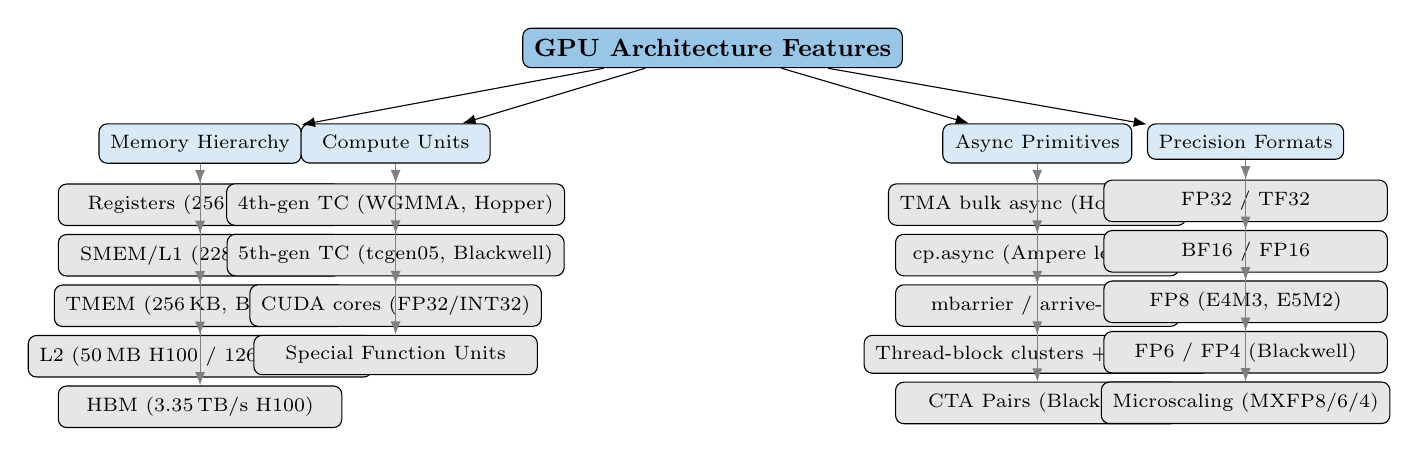
\begin{tikzpicture}[
  node distance=0.35cm and 0.5cm,
  box/.style={draw, rounded corners=3pt, font=\scriptsize, inner sep=4pt, text centered, minimum width=3.2cm},
  catbox/.style={box, fill=hopperblue!15, minimum width=2.4cm},
  itembox/.style={box, fill=lightgray, minimum width=3.6cm},
  rootbox/.style={box, fill=hopperblue!40, font=\small\bfseries, minimum width=3cm},
]
% Root
\node[rootbox] (root) {GPU Architecture Features};

% Categories
\node[catbox, below left=0.7cm and 2.8cm of root] (mem) {Memory Hierarchy};
\node[catbox, below left=0.7cm and 0.4cm of root] (comp) {Compute Units};
\node[catbox, below right=0.7cm and 0.5cm of root] (async) {Async Primitives};
\node[catbox, below right=0.7cm and 3.1cm of root] (prec) {Precision Formats};

% Memory items
\node[itembox, below=0.25cm of mem] (r1) {Registers (256\,KB/SM)};
\node[itembox, below=0.1cm of r1] (r2) {SMEM/L1 (228\,KB/SM)};
\node[itembox, below=0.1cm of r2] (r3) {TMEM (256\,KB, Blackwell)};
\node[itembox, below=0.1cm of r3] (r4) {L2 (50\,MB H100 / 126\,MB B200)};
\node[itembox, below=0.1cm of r4] (r5) {HBM (3.35\,TB/s H100)};

% Compute items
\node[itembox, below=0.25cm of comp] (c1) {4th-gen TC (WGMMA, Hopper)};
\node[itembox, below=0.1cm of c1] (c2) {5th-gen TC (tcgen05, Blackwell)};
\node[itembox, below=0.1cm of c2] (c3) {CUDA cores (FP32/INT32)};
\node[itembox, below=0.1cm of c3] (c4) {Special Function Units};

% Async items
\node[itembox, below=0.25cm of async] (a1) {TMA bulk async (Hopper+)};
\node[itembox, below=0.1cm of a1] (a2) {cp.async (Ampere legacy)};
\node[itembox, below=0.1cm of a2] (a3) {mbarrier / arrive-wait};
\node[itembox, below=0.1cm of a3] (a4) {Thread-block clusters + DSMEM};
\node[itembox, below=0.1cm of a4] (a5) {CTA Pairs (Blackwell)};

% Precision items
\node[itembox, below=0.25cm of prec] (p1) {FP32 / TF32};
\node[itembox, below=0.1cm of p1] (p2) {BF16 / FP16};
\node[itembox, below=0.1cm of p2] (p3) {FP8 (E4M3, E5M2)};
\node[itembox, below=0.1cm of p3] (p4) {FP6 / FP4 (Blackwell)};
\node[itembox, below=0.1cm of p4] (p5) {Microscaling (MXFP8/6/4)};

% Edges root -> categories
\draw[-{Latex}] (root) -- (mem);
\draw[-{Latex}] (root) -- (comp);
\draw[-{Latex}] (root) -- (async);
\draw[-{Latex}] (root) -- (prec);

% Edges categories -> items
\foreach \cat/\items in {mem/{r1,r2,r3,r4,r5}, comp/{c1,c2,c3,c4}, async/{a1,a2,a3,a4,a5}, prec/{p1,p2,p3,p4,p5}}{
  \foreach \item in \items {
    \draw[-{Latex}, gray] (\cat) -- (\item);
  }
}
\end{tikzpicture}
\caption{Taxonomy of GPU architecture features relevant to MoE kernel optimization on Hopper and Blackwell. Features marked ``Blackwell'' are new in the B200 generation.}
\label{fig:hw-taxonomy}
\end{figure}

\subsection{The GPU Memory Hierarchy}
\label{sec:hw-memhier}

GPU performance is governed, more than anything else, by the steep bandwidth gradient between successive levels of the memory hierarchy. On an H100 SXM5 GPU, register files deliver effectively unlimited bandwidth (the compiler aggressively allocates intermediate values to registers), shared memory (SMEM) provides roughly 19\,TB/s of bandwidth per SM aggregated across the whole chip, the unified L2 cache delivers roughly 12\,TB/s, and HBM3 delivers 3.35\,TB/s. Blackwell's B200 widens the gradient further: HBM3e bandwidth grows to 8\,TB/s, and the L2 cache grows from 50\,MB to 126\,MB \citep{nvidia2022hopper,nvidia2024blackwell}. The fundamental design problem for any high-performance kernel is to keep working data as close to the registers as possible and to reuse it as many times as possible before evicting it.

This problem is most usefully analyzed through the \emph{roofline model} \citep{williams2009roofline}, which plots achievable throughput as a function of arithmetic intensity (FLOPs per byte of memory traffic). For a given precision, every kernel sits somewhere on a piecewise-linear curve: at low arithmetic intensity, throughput is limited by the slope of the bandwidth roof; at high arithmetic intensity, it is capped by the horizontal compute roof. The transition point---the arithmetic intensity at which a kernel becomes compute-bound rather than memory-bound---is determined by the ratio of peak compute to peak bandwidth. On H100 in BF16, that ratio is roughly 295 FLOPs/byte; in FP8 it doubles to roughly 590 FLOPs/byte; on B200 in FP4 it climbs higher still. The practical consequence is that as tensor cores get faster, more and more workloads slip into the memory-bound region, and kernel design becomes dominated by data-movement decisions rather than instruction-issue decisions \citep{boehm2022cudammm,gordic2024matmul}.

MoE workloads sit in an awkward part of this curve. A standard dense matmul of large square matrices is comfortably compute-bound on Hopper, but MoE introduces three pathologies that pull effective arithmetic intensity downward. First, routing partitions tokens into per-expert groups whose sizes vary at runtime, so each expert sees a relatively small (sometimes very small) effective $M$ dimension and the per-expert matmul is closer to the memory-bound regime. Second, MoE forward passes typically launch two GEMMs per layer (up-projection followed by down-projection) with an intermediate activation that, if naively materialized, must be written to HBM and read back. Third, the routing metadata itself---expert offsets, gather indices, expert frequencies---is small but accessed twice (once per GEMM). Each of these issues is addressable, and the rest of this survey is in large part a catalogue of how. But all of them depend on the kernel writer having a precise mental model of the memory hierarchy they are programming against.

\begin{figure}[t]
\centering
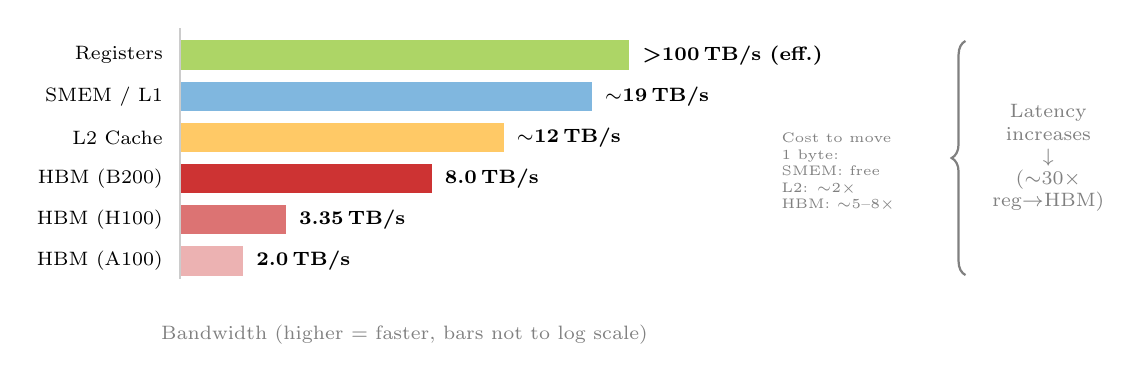
\begin{tikzpicture}[scale=0.95]
  % Memory hierarchy pyramid / stacked bars
  % X: level name, Y: bandwidth (log scale conceptually shown as bar heights)
  % We draw a horizontal bar chart with annotated bandwidth values

  % Define levels and their data
  % Rows: Registers, SMEM, L2, HBM (A100), HBM (H100), HBM (B200)
  \def\bw{5.5} % total width of chart area

  % Color coding
  \colorlet{regcol}{nvidiagreen!60}
  \colorlet{smemcol}{hopperblue!50}
  \colorlet{l2col}{ambercolor!60}
  \colorlet{hbma100}{blackwellred!30}
  \colorlet{hbmh100}{blackwellred!55}
  \colorlet{hbmb200}{blackwellred!80}

  % --- horizontal bar chart ---
  % Each bar: (y position, label, bar width scaled, color, annotation)
  % BW values: Registers ~unlimited (shown as 100x), SMEM~19 TB/s, L2~12 TB/s, HBM A100 2.0, H100 3.35, B200 8.0
  % Scale: log-ish, normalized to HBM-H100=1.0 unit = 1.6cm
  \def\unit{0.42} % 1 TB/s = this many cm

  % SMEM: ~19 TB/s -> 7.98cm, cap at 6cm with ">" indicator
  % L2: ~12 TB/s -> 5.04cm
  % HBM A100: 2.0 -> 0.84cm
  % HBM H100: 3.35 -> 1.41cm
  % HBM B200: 8.0 -> 3.36cm
  % Registers: "unlimited" -> use 6cm with annotation

  \def\yspace{0.55}
  \def\barh{0.38}

  % Draw bars
  \filldraw[regcol] (0, 6*\yspace) rectangle (6.0, 6*\yspace+\barh);
  \filldraw[smemcol] (0, 5*\yspace) rectangle (5.5, 5*\yspace+\barh);
  \filldraw[l2col] (0, 4*\yspace) rectangle (4.32, 4*\yspace+\barh);
  \filldraw[hbmb200] (0, 3*\yspace) rectangle (3.36, 3*\yspace+\barh);
  \filldraw[hbmh100] (0, 2*\yspace) rectangle (1.41, 2*\yspace+\barh);
  \filldraw[hbma100] (0, 1*\yspace) rectangle (0.84, 1*\yspace+\barh);

  % Row labels (left side)
  \node[font=\scriptsize, anchor=east] at (-0.1, 6*\yspace+\barh/2) {Registers};
  \node[font=\scriptsize, anchor=east] at (-0.1, 5*\yspace+\barh/2) {SMEM / L1};
  \node[font=\scriptsize, anchor=east] at (-0.1, 4*\yspace+\barh/2) {L2 Cache};
  \node[font=\scriptsize, anchor=east] at (-0.1, 3*\yspace+\barh/2) {HBM (B200)};
  \node[font=\scriptsize, anchor=east] at (-0.1, 2*\yspace+\barh/2) {HBM (H100)};
  \node[font=\scriptsize, anchor=east] at (-0.1, 1*\yspace+\barh/2) {HBM (A100)};

  % Value annotations (right side)
  \node[font=\scriptsize\bfseries, anchor=west] at (6.05, 6*\yspace+\barh/2) {\textgreater{}100\,TB/s (eff.)};
  \node[font=\scriptsize\bfseries, anchor=west] at (5.55, 5*\yspace+\barh/2) {$\sim$19\,TB/s};
  \node[font=\scriptsize\bfseries, anchor=west] at (4.37, 4*\yspace+\barh/2) {$\sim$12\,TB/s};
  \node[font=\scriptsize\bfseries, anchor=west] at (3.41, 3*\yspace+\barh/2) {8.0\,TB/s};
  \node[font=\scriptsize\bfseries, anchor=west] at (1.46, 2*\yspace+\barh/2) {3.35\,TB/s};
  \node[font=\scriptsize\bfseries, anchor=west] at (0.89, 1*\yspace+\barh/2) {2.0\,TB/s};

  % X axis label
  \node[font=\scriptsize, gray] at (3, -0.25) {Bandwidth (higher = faster, bars not to log scale)};

  % Vertical divider lines for visual clarity
  \draw[gray!40, thin] (0, 0.5) -- (0, 7*\yspace);

  % Latency annotation on right
  \draw[decorate, decoration={brace, amplitude=5pt}, thick, gray]
    (10.5, 1*\yspace) -- (10.5, 6*\yspace+\barh)
    node[midway, right=6pt, font=\scriptsize, align=center] {Latency\\increases\\$\downarrow$\\($\sim$30$\times$\\reg$\to$HBM)};

  % Cost-to-move annotation
  \node[font=\tiny, gray, align=left] at (8.8, 3.5*\yspace) {Cost to move\\1 byte:\\SMEM: free\\L2: $\sim$2$\times$\\HBM: $\sim$5--8$\times$};
\end{tikzpicture}
\caption{GPU memory hierarchy bandwidth on H100 SXM5 and B200. Effective register bandwidth exceeds HBM by $>$30$\times$; each level down the hierarchy adds latency and reduces bandwidth. The fundamental objective of high-performance kernel engineering is to keep hot data in the highest level possible. SMEM and L2 bandwidth figures are aggregate (chip-wide); register bandwidth per SM is even higher.}
\label{fig:mem-hierarchy}
\end{figure}

\subsection{NVIDIA Hopper (H100)}
\label{sec:hw-hopper}

The H100 GPU \citep{nvidia2022hopper}, launched in 2022, introduced four hardware features that have collectively defined the post-Ampere style of high-performance kernel writing: warp-group MMA (WGMMA), the Tensor Memory Accelerator (TMA), thread block clusters with distributed shared memory, and FP8 tensor cores. We discuss each in turn, then describe the producer-consumer warp-specialization pattern that ties them together \citep{luo2024hopperdissect}.

\subsubsection{Warp-Group MMA (WGMMA)}
On Ampere, tensor-core matmul instructions (\texttt{mma.sync}) operated at the granularity of a single warp and were synchronous: the warp issuing the instruction stalled until the result was available in registers. Hopper's 4th-generation tensor cores expose a new \texttt{wgmma.mma\_async} instruction family that operates at the granularity of an entire \emph{warp group} (four warps, 128 threads) and is fully asynchronous. A single WGMMA instruction can compute a $64 \times N \times 16$ tile of $C = A \cdot B + C$ for $N \in \{8, 16, \ldots, 256\}$, with the accumulator held in registers. The instruction returns immediately; the warp group must later wait on a fence (\texttt{wgmma.wait\_group}) to ensure the result is visible. The asynchronous nature is essential: it allows the same warp group to issue subsequent loads, prepare the next tile, or even issue more WGMMAs while previous ones are in flight. This is the building block on which every Hopper-native matmul kernel depends \citep{thakkar2023cutlass,shah2024flashattention3}.

A second crucial detail is that the $A$ operand for WGMMA can be sourced either from registers or directly from shared memory via descriptor tables, while the $B$ operand must come from shared memory. This SMEM-resident operand model interacts directly with TMA: the canonical pattern is for TMA to bulk-load tiles of $A$ and $B$ into SMEM, and for WGMMA to consume them in place without ever transiting through registers.

\subsubsection{Tensor Memory Accelerator (TMA)}
Ampere introduced \texttt{cp.async}, a per-thread asynchronous global-to-shared copy instruction that allowed kernels to overlap memory loads with compute. Hopper replaces this with the Tensor Memory Accelerator, a dedicated hardware unit that performs \emph{bulk} async copies described by tile descriptors. A single \texttt{cp.async.bulk.tensor} instruction issued by one thread can move an entire multidimensional tile of tens of kilobytes between HBM and SMEM, with the address arithmetic, boundary handling, and coordinate translation all performed in hardware. TMA also supports multicast, in which a single load is broadcast to the SMEM of multiple CTAs in a thread block cluster, eliminating redundant HBM traffic when several CTAs need the same tile.

The descriptor model is worth dwelling on. Rather than computing addresses in software, the kernel sets up a \texttt{CUtensorMap} descriptor describing the tensor's shape, strides, element size, swizzle pattern, and out-of-bounds fill value, and then issues TMA loads by specifying tile coordinates. This eliminates a long tail of address-arithmetic instructions from the kernel's hot path and frees up registers and instruction issue slots for compute. The combination of WGMMA and TMA is what makes Hopper kernels look so different from Ampere kernels: the inner loop is dominated by descriptor loads, barrier waits, and WGMMA issues, with very little explicit address computation.

\subsubsection{Thread Block Clusters and Distributed Shared Memory}
Hopper introduces a new level of the execution hierarchy above the thread block: the \emph{thread block cluster}, a group of up to 16 CTAs that are co-scheduled on neighboring SMs and that can directly access each other's shared memory. This region is referred to as Distributed Shared Memory (DSMEM). For matmul kernels, clusters enable a form of cooperative tiling in which several CTAs share the cost of loading a common operand tile via TMA multicast, then consume it from their local SMEM views. The synchronization primitive that makes this work is the cluster-scope barrier, an extension of the \texttt{mbarrier} mechanism that allows arrive-wait synchronization across CTAs in the cluster.

\subsubsection{FP8 and the Transformer Engine}
Hopper's tensor cores natively support FP8 in two formats: E4M3 (4 exponent bits, 3 mantissa bits) for forward activations and weights, and E5M2 (5 exponent bits, 2 mantissa bits) for gradients during backpropagation. Peak FP8 throughput is double FP16 throughput, making FP8 attractive for both training and inference if numerical stability can be maintained. The Transformer Engine library \citep{nvidia2024transformerengine} provides automatic tensor scaling: it tracks the dynamic range of activations during training and rescales tensors before each tensor-core operation to keep values within FP8's representable range.

\subsubsection{The Producer-Consumer Warp-Specialization Pattern}
The four features above are most powerful when combined into the producer-consumer warp-specialization pattern that has become the canonical Hopper kernel idiom \citep{shah2024flashattention3,thakkar2023cutlass,colfax2024fa3}. A typical Hopper matmul kernel allocates one warp group as the \emph{producer}, whose only job is to issue TMA loads of operand tiles into a circular buffer in SMEM, and one or more warp groups as \emph{consumers}, which issue WGMMAs against tiles already loaded by the producer. Synchronization between producer and consumer is mediated by \texttt{mbarrier} arrive-wait pairs: the producer increments a barrier after each TMA load completes, and the consumer waits on the barrier before issuing the corresponding WGMMA. Because TMA, WGMMA, and barrier waits are all asynchronous, the producer and consumer can run in lockstep without ever stalling on each other, achieving close to 100\% tensor-core utilization on suitably shaped problems. A common refinement is \emph{ping-pong scheduling}, in which two consumer warp groups alternate so that one is in its epilogue while the other is in its mainloop, hiding the cost of writing results to SMEM.

\begin{figure}[t]
\centering
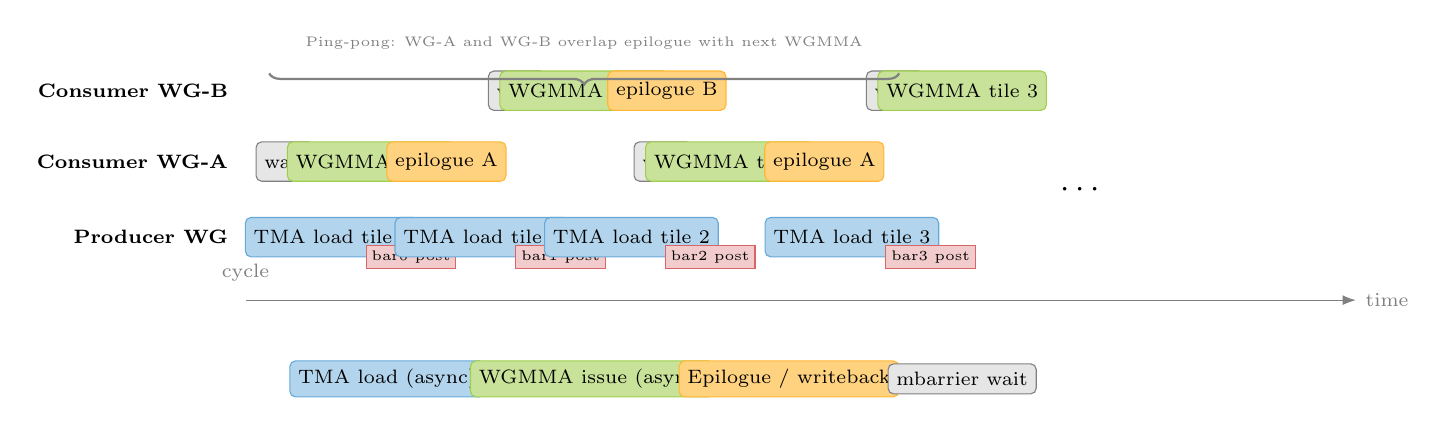
\begin{tikzpicture}[
  tmabox/.style={fill=hopperblue!30, draw=hopperblue!60, rounded corners=2pt, font=\scriptsize, inner sep=3pt},
  wgmmabox/.style={fill=nvidiagreen!40, draw=nvidiagreen!70, rounded corners=2pt, font=\scriptsize, inner sep=3pt},
  epilbox/.style={fill=ambercolor!50, draw=ambercolor!80, rounded corners=2pt, font=\scriptsize, inner sep=3pt},
  waitbox/.style={fill=lightgray, draw=gray, rounded corners=2pt, font=\scriptsize, inner sep=3pt},
  barrbox/.style={fill=blackwellred!20, draw=blackwellred!60, font=\tiny, inner sep=2pt},
]
\def\T{1.6} % tile width
\def\gap{0.06}
\def\yscale{0.6}

% Time axis
\draw[-{Latex}, gray] (-0.3, 0) -- (13.8, 0) node[right, font=\scriptsize] {time};
\node[font=\scriptsize, gray] at (-0.3, 0.35) {cycle};

% Row labels
\node[font=\scriptsize\bfseries, anchor=east] at (-0.4, 1*\yscale+0.2) {Producer WG};
\node[font=\scriptsize\bfseries, anchor=east] at (-0.4, 2.6*\yscale+0.2) {Consumer WG-A};
\node[font=\scriptsize\bfseries, anchor=east] at (-0.4, 4.1*\yscale+0.2) {Consumer WG-B};

% === Tile 0 ===
\node[tmabox, minimum width=\T cm, minimum height=0.5cm] at (0.8, 1*\yscale+0.2) {TMA load tile 0};
\node[barrbox] at (1.8, 0.55) {bar0 post};

\node[waitbox, minimum width=0.4cm, minimum height=0.5cm] at (0.2, 2.6*\yscale+0.2) {wait};
\node[wgmmabox, minimum width=\T cm, minimum height=0.5cm] at (1.3, 2.6*\yscale+0.2) {WGMMA tile 0};

% === Tile 1 ===
\node[tmabox, minimum width=\T cm, minimum height=0.5cm] at (2.7, 1*\yscale+0.2) {TMA load tile 1};
\node[barrbox] at (3.7, 0.55) {bar1 post};

\node[epilbox, minimum width=0.9cm, minimum height=0.5cm] at (2.25, 2.6*\yscale+0.2) {epilogue A};
\node[waitbox, minimum width=0.3cm, minimum height=0.5cm] at (3.15, 4.1*\yscale+0.2) {wait};
\node[wgmmabox, minimum width=\T cm, minimum height=0.5cm] at (4.0, 4.1*\yscale+0.2) {WGMMA tile 1};

% === Tile 2 ===
\node[tmabox, minimum width=\T cm, minimum height=0.5cm] at (4.6, 1*\yscale+0.2) {TMA load tile 2};
\node[barrbox] at (5.6, 0.55) {bar2 post};

\node[waitbox, minimum width=0.3cm, minimum height=0.5cm] at (5.0, 2.6*\yscale+0.2) {wait};
\node[wgmmabox, minimum width=\T cm, minimum height=0.5cm] at (5.85, 2.6*\yscale+0.2) {WGMMA tile 2};
\node[epilbox, minimum width=0.9cm, minimum height=0.5cm] at (5.05, 4.1*\yscale+0.2) {epilogue B};

% === Tile 3 ===
\node[tmabox, minimum width=\T cm, minimum height=0.5cm] at (7.4, 1*\yscale+0.2) {TMA load tile 3};
\node[barrbox] at (8.4, 0.55) {bar3 post};

\node[epilbox, minimum width=0.9cm, minimum height=0.5cm] at (7.05, 2.6*\yscale+0.2) {epilogue A};
\node[waitbox, minimum width=0.3cm, minimum height=0.5cm] at (7.95, 4.1*\yscale+0.2) {wait};
\node[wgmmabox, minimum width=\T cm, minimum height=0.5cm] at (8.8, 4.1*\yscale+0.2) {WGMMA tile 3};

% Ellipsis
\node[font=\large] at (10.3, 2*\yscale+0.2) {$\cdots$};

% Legend
\begin{scope}[shift={(0,-1.0)}]
  \node[tmabox, minimum width=1.8cm] at (1.5, 0) {TMA load (async)};
  \node[wgmmabox, minimum width=2.0cm] at (4.1, 0) {WGMMA issue (async)};
  \node[epilbox, minimum width=1.6cm] at (6.6, 0) {Epilogue / writeback};
  \node[waitbox, minimum width=1.3cm] at (8.8, 0) {mbarrier wait};
\end{scope}

% Braces for ping-pong annotation
\draw[decorate, decoration={brace, amplitude=4pt, mirror}, thick, gray]
  (0.0, 4.8*\yscale) -- (8.0, 4.8*\yscale)
  node[midway, above=5pt, font=\tiny, gray] {Ping-pong: WG-A and WG-B overlap epilogue with next WGMMA};
\end{tikzpicture}
\caption{Hopper producer-consumer warp-specialization pipeline with ping-pong scheduling. The Producer warp group issues asynchronous TMA loads into SMEM double-buffers and posts \texttt{mbarrier} signals. Two Consumer warp groups (WG-A, WG-B) wait on the barrier then issue WGMMA tiles; they alternate so that one is in its epilogue (writing accumulator to SMEM/HBM) while the other is computing, hiding epilogue latency behind tensor-core throughput.}
\label{fig:warp-spec}
\end{figure}

\subsection{NVIDIA Blackwell (B200/GB200)}
\label{sec:hw-blackwell}

Blackwell, launched in 2024, builds on the Hopper foundation with three significant architectural changes: a new generation of tensor cores accessed via \texttt{tcgen05} instructions, a dedicated Tensor Memory (TMEM) space, and CTA pairs that allow two CTAs to cooperate on a single tensor-core instruction \citep{nvidia2024blackwell}. The B200 die also expands the L2 cache to 126\,MB, increases HBM3e bandwidth to 8\,TB/s, and adds native support for FP4 and FP6 microscaling formats. We discuss each change.

\subsubsection{5th-Generation Tensor Cores and tcgen05}
The new \texttt{tcgen05.mma} instruction family is, in spirit, a successor to WGMMA: it is asynchronous, operates on large tile shapes, and is designed to be issued from a coordinated group of warps. The most important change relative to WGMMA is where the accumulator lives. WGMMA holds its accumulator in registers, which constrains tile sizes (large tiles consume many registers per warp) and creates pressure on the register file. \texttt{tcgen05.mma}, by contrast, places its accumulator in a new on-chip memory called Tensor Memory.

\subsubsection{Tensor Memory (TMEM)}
Tensor Memory is a dedicated 256\,KB-per-SM on-chip memory, distinct from both registers and shared memory. It is addressable only by tcgen05 instructions and a small set of accompanying load/store instructions (\texttt{tcgen05.alloc}, \texttt{tcgen05.ld}, \texttt{tcgen05.st}). The motivation is simple: by moving the matmul accumulator out of registers, Blackwell removes the register-pressure constraint that limited tile sizes on Hopper, allowing larger and more efficient tile shapes. The cost is added kernel-design complexity, because TMEM must be explicitly allocated, managed, and freed, and because data must be staged through SMEM to and from TMEM rather than flowing directly through registers as on Hopper. Early kernel writers have found that the ergonomic differences between Hopper and Blackwell are larger than the differences between Volta and Hopper, despite the fact that the underlying compute model is conceptually similar \citep{veitner2025blackwell}.

\subsubsection{CTA Pairs}
Blackwell allows two CTAs from the same cluster to be \emph{paired}: a single \texttt{tcgen05.mma} instruction can be issued cooperatively by both CTAs, with operands sourced from one CTA's SMEM and the accumulator residing in the other CTA's TMEM. This effectively doubles the effective shared memory available to a single tensor-core instruction and enables larger tile shapes than a single CTA could support.

\subsubsection{FP4, FP6, and Microscaling}
Blackwell adds tensor-core support for FP4 and FP6 in addition to FP8. The peak throughput in FP4 is roughly $2\times$ FP8 and $4\times$ FP16, making FP4 enormously attractive for inference and increasingly viable for training. To maintain numerical stability at such low precision, Blackwell supports \emph{microscaling} formats (MXFP8, MXFP6, MXFP4) in which a small block of values (typically 32 elements) shares a single FP8 scale factor. Microscaling is a hardware-level extension of the per-tensor scaling that the Transformer Engine performs in software on Hopper, and it brings dramatically finer-grained dynamic range control \citep{rouhani2023microscaling}.

\subsubsection{L2 Cache and the Persistent-Kernel Sweet Spot}
The 126\,MB L2 cache on B200 is more than $2.5\times$ the size of H100's L2. This changes the kernel-design sweet spot in two ways. First, larger weight tiles fit in L2, making rasterized tile schedules more effective and increasing the effective L2 hit rate for grouped GEMMs. Second, intermediate activations that are too large to fit in L2 on H100 (such as the $\sim$32\,MB Y1 tensor in a typical MoE forward pass) now fit comfortably, opening the door to L2-cache-warm kernel fusion patterns that we discuss in detail in Section~\ref{sec:fusion}.

\subsection{Hardware Comparison}
\label{sec:hw-comparison}

Table~\ref{tab:hw-detailed} summarizes the hardware features of A100, H100 SXM5, and B200, focusing on the dimensions that matter for MoE kernel design. The progression from A100 to H100 introduced asynchronous tensor cores and bulk async copy; the progression from H100 to B200 introduced dedicated accumulator memory and a roughly $2.5\times$ growth in L2 cache. Both transitions also brought lower-precision tensor-core formats whose effective use depends on careful kernel-level engineering.

\begin{table}[t]
\caption{Hardware comparison of A100, H100 SXM5, and B200. SMEM and L1 share the same physical storage on Ampere/Hopper. TMEM is a new Blackwell-only memory space. TFLOP figures are dense tensor-core peaks; sparse peaks are roughly $2\times$ higher.}
\label{tab:hw-detailed}
\centering\small
\begin{tabular}{lccc}
\toprule
Feature & A100 SXM4 & H100 SXM5 & B200 \\
\midrule
SM count & 108 & 132 & 160 (per die, $\times 2$) \\
Register file / SM & 256\,KB & 256\,KB & 256\,KB \\
SMEM + L1 / SM & 192\,KB & 228\,KB & 228\,KB \\
TMEM / SM & --- & --- & 256\,KB \\
L2 cache & 40\,MB & 50\,MB & 126\,MB \\
HBM capacity & 80\,GB & 80\,GB & 192\,GB \\
HBM bandwidth & 2.0\,TB/s & 3.35\,TB/s & 8.0\,TB/s \\
Tensor core gen & 3rd & 4th (WGMMA) & 5th (tcgen05) \\
BF16 dense TFLOPs & 312 & 989 & $\sim$2,250 \\
FP8 dense TFLOPs & --- & 1,979 & $\sim$4,500 \\
FP4 dense TFLOPs & --- & --- & $\sim$9,000 \\
NVLink bandwidth & 600\,GB/s & 900\,GB/s & 1,800\,GB/s \\
\bottomrule
\end{tabular}
\end{table}

The single most important takeaway from Table~\ref{tab:hw-detailed} for the rest of this survey is that the ratio of compute throughput to HBM bandwidth has grown substantially with each generation. On A100 in BF16, this ratio is approximately 156 FLOPs/byte; on H100 in BF16, 295 FLOPs/byte; on B200 in BF16, roughly 280 FLOPs/byte (compute and bandwidth grew in tandem); but in FP8 on H100 it is 590 FLOPs/byte and in FP4 on B200 it exceeds 1,100 FLOPs/byte. As the precision drops, more and more workloads slip from compute-bound into memory-bound territory, making kernel-level data-movement optimization the dominant lever for end-to-end performance. This is the technical context in which the techniques surveyed in Sections~\ref{sec:matmul} through \ref{sec:fusion} should be understood.

\begin{figure}[t]
\centering
\begin{tikzpicture}
\begin{loglogaxis}[
  width=12cm, height=7cm,
  xlabel={Arithmetic Intensity (FLOPs/byte)},
  ylabel={Throughput (TFLOPS)},
  xmin=1, xmax=5000,
  ymin=10, ymax=20000,
  grid=both,
  grid style={gray!20},
  legend style={at={(0.03,0.97)}, anchor=north west, font=\scriptsize, fill=white, draw=gray},
  tick label style={font=\scriptsize},
  label style={font=\small},
  title style={font=\small},
  title={Roofline Model: A100, H100, B200},
]

% --- A100 BF16 roof: 312 TFLOPS, BW=2.0 TB/s, ridge=312/2=156 ---
\addplot[thick, hbma100!80!black, domain=1:156] {2.0*x};
\addplot[thick, hbma100!80!black, domain=156:5000] {312};
\addlegendentry{A100 BF16 (312 TFLOPS, 2.0 TB/s)}

% --- H100 BF16 roof: 989 TFLOPS, BW=3.35 TB/s, ridge=989/3.35≈295 ---
\addplot[thick, hopperblue, domain=1:295] {3.35*x};
\addplot[thick, hopperblue, domain=295:5000] {989};
\addlegendentry{H100 BF16 (989 TFLOPS, 3.35 TB/s)}

% --- H100 FP8 roof: 1979 TFLOPS, BW=3.35 TB/s, ridge=1979/3.35≈590 ---
\addplot[thick, hopperblue, dashed, domain=1:590] {3.35*x};
\addplot[thick, hopperblue, dashed, domain=590:5000] {1979};
\addlegendentry{H100 FP8 (1979 TFLOPS, 3.35 TB/s)}

% --- B200 BF16 roof: ~2250 TFLOPS, BW=8.0 TB/s, ridge=2250/8=281 ---
\addplot[thick, blackwellred, domain=1:281] {8.0*x};
\addplot[thick, blackwellred, domain=281:5000] {2250};
\addlegendentry{B200 BF16 ($\approx$2250 TFLOPS, 8.0 TB/s)}

% --- B200 FP4 roof: ~9000 TFLOPS, BW=8.0 TB/s, ridge=9000/8=1125 ---
\addplot[thick, blackwellred, dashed, domain=1:1125] {8.0*x};
\addplot[thick, blackwellred, dashed, domain=1125:5000] {9000};
\addlegendentry{B200 FP4 ($\approx$9000 TFLOPS, 8.0 TB/s)}

% --- Annotate workload points ---
% Dense GEMM (large square, BF16, H100): ~295 FLOPs/byte -> compute-bound
\addplot[only marks, mark=*, mark size=3pt, hopperblue] coordinates {(295, 850)};
\node[font=\tiny, hopperblue, anchor=south] at (axis cs:295, 870) {Dense GEMM};

% MoE grouped GEMM (small m_e, BF16, H100): ~30 FLOPs/byte -> mem-bound
\addplot[only marks, mark=square*, mark size=3pt, ambercolor!80!black] coordinates {(30, 100)};
\node[font=\tiny, ambercolor!80!black, anchor=north] at (axis cs:30, 95) {MoE GEMM (small $m_e$)};

% Attention FA3 (H100, BF16): ~50 FLOPs/byte (IO-aware, effective)
\addplot[only marks, mark=triangle*, mark size=3pt, nvidiagreen!70!black] coordinates {(50, 167)};
\node[font=\tiny, nvidiagreen!70!black, anchor=west] at (axis cs:52, 167) {FA3 attn.};

\end{loglogaxis}
\end{tikzpicture}
\caption{Roofline model for A100, H100 SXM5, and B200. Solid lines show BF16 roofs; dashed lines show FP8 (H100) and FP4 (B200) roofs. Annotated points show representative achieved throughput for a well-tuned dense GEMM (compute-bound), an MoE grouped GEMM with small per-expert token count (memory-bound), and FA3 attention. As precision drops from BF16 to FP8/FP4, the ridge point shifts right, pushing more workloads into the memory-bound regime and increasing the importance of data-movement optimization.}
\label{fig:roofline}
\end{figure}

\section{The Matmul Kernel Engineering Lineage}
\label{sec:matmul}

Matrix multiplication is the workhorse of every Transformer, and grouped variants of matmul are the workhorse of every MoE layer. The history of high-performance GPU matmul is therefore the prehistory of high-performance MoE kernels. This section traces that lineage from the earliest pedagogical CUDA optimizations through modern tile-based DSLs, with particular attention to how each new layer of abstraction has changed what kernels are practical to write and how close to peak hardware utilization they can get. Figure~\ref{fig:matmul-taxonomy} organizes the approaches into a taxonomy.

\begin{figure}[t]
\centering
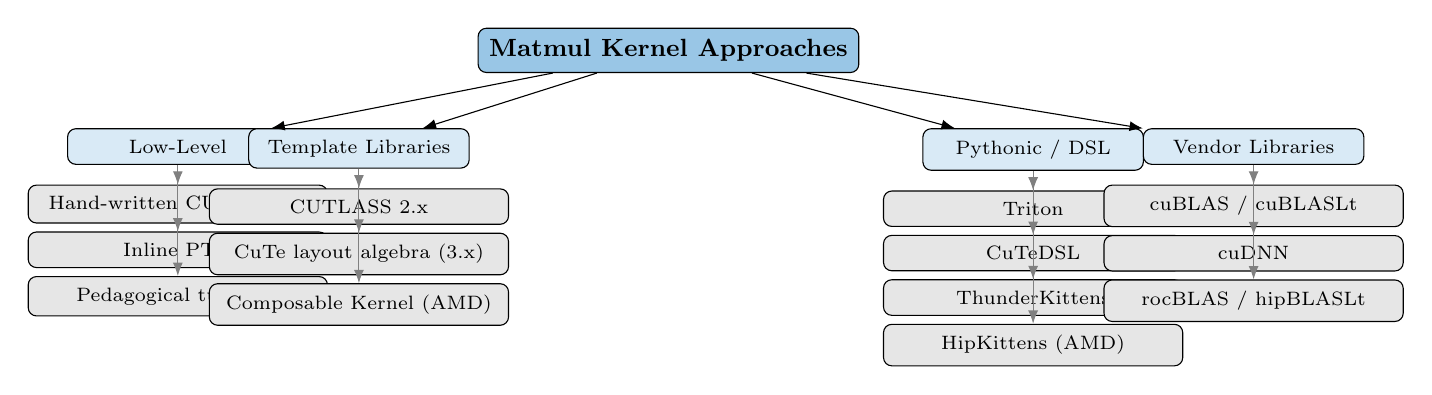
\begin{tikzpicture}[
  node distance=0.3cm and 0.5cm,
  box/.style={draw, rounded corners=3pt, font=\scriptsize, inner sep=4pt, text centered, minimum width=3.8cm},
  catbox/.style={box, fill=hopperblue!15, minimum width=2.8cm},
  itembox/.style={box, fill=lightgray, minimum width=3.8cm},
  rootbox/.style={box, fill=hopperblue!40, font=\small\bfseries, minimum width=3.2cm},
]
\node[rootbox] (root) {Matmul Kernel Approaches};

\node[catbox, below left=0.7cm and 2.4cm of root] (ll) {Low-Level};
\node[catbox, below left=0.7cm and 0.1cm of root] (tl) {Template Libraries};
\node[catbox, below right=0.7cm and 0.8cm of root] (dsl) {Pythonic / DSL};
\node[catbox, below right=0.7cm and 3.6cm of root] (vl) {Vendor Libraries};

\node[itembox, below=0.25cm of ll] (l1) {Hand-written CUDA C++};
\node[itembox, below=0.1cm of l1] (l2) {Inline PTX};
\node[itembox, below=0.1cm of l2] (l3) {Pedagogical tutorials};

\node[itembox, below=0.25cm of tl] (t1) {CUTLASS 2.x};
\node[itembox, below=0.1cm of t1] (t2) {CuTe layout algebra (3.x)};
\node[itembox, below=0.1cm of t2] (t3) {Composable Kernel (AMD)};

\node[itembox, below=0.25cm of dsl] (d1) {Triton};
\node[itembox, below=0.1cm of d1] (d2) {CuTeDSL};
\node[itembox, below=0.1cm of d2] (d3) {ThunderKittens};
\node[itembox, below=0.1cm of d3] (d4) {HipKittens (AMD)};

\node[itembox, below=0.25cm of vl] (v1) {cuBLAS / cuBLASLt};
\node[itembox, below=0.1cm of v1] (v2) {cuDNN};
\node[itembox, below=0.1cm of v2] (v3) {rocBLAS / hipBLASLt};

\draw[-{Latex}] (root) -- (ll);
\draw[-{Latex}] (root) -- (tl);
\draw[-{Latex}] (root) -- (dsl);
\draw[-{Latex}] (root) -- (vl);

\foreach \cat/\items in {ll/{l1,l2,l3}, tl/{t1,t2,t3}, dsl/{d1,d2,d3,d4}, vl/{v1,v2,v3}}{
  \foreach \item in \items {
    \draw[-{Latex}, gray] (\cat) -- (\item);
  }
}
\end{tikzpicture}
\caption{Taxonomy of matmul kernel implementation approaches, ordered roughly by abstraction level. HipKittens targets AMD CDNA hardware; all others target NVIDIA.}
\label{fig:matmul-taxonomy}
\end{figure}

\subsection{The Pedagogical Progression}
\label{sec:matmul-pedagogy}

Before discussing libraries and DSLs, it is worth recalling the optimization steps that any high-performance matmul kernel must perform, because they shape every higher-level abstraction. Simon Boehm's widely-cited tutorial \citep{boehm2022cudammm} walks through ten successive versions of a square FP32 matmul kernel on an A6000 GPU, starting from a naive global-memory implementation that achieves roughly 1\% of cuBLAS performance and ending with a hand-tuned kernel that matches cuBLAS within a few percent. The optimization steps are, in order: (1) coalesced global memory access, so that consecutive threads in a warp load consecutive addresses; (2) shared-memory tiling, so that each tile of $A$ and $B$ is loaded once from HBM and reused across multiple output elements; (3) one-dimensional thread tiling, in which each thread computes multiple output elements; (4) two-dimensional thread tiling, which further amortizes shared-memory loads; (5) vectorized loads using \texttt{LDG.E.128} (128-bit loads), which improve memory throughput; (6) avoidance of shared-memory bank conflicts via padding or swizzling; (7) auto-tuning of tile sizes; (8) warptiling, which adds an intermediate level of partitioning between threadblock and thread; (9) double buffering to hide global-memory latency behind compute; and (10) restructuring for tensor cores. Aleksa Gordic's matmul tutorial \citep{gordic2024matmul} covers similar ground with a complementary emphasis on the roofline model and the relationship between arithmetic intensity and tile size.

These tutorials are worth studying not because anyone should write matmul kernels this way today---vendor libraries and high-level DSLs almost always do better with less effort---but because every higher-level abstraction is, internally, a more elegant repackaging of these same optimization steps. CUTLASS templates encode them as compile-time parameters; CuTe encodes them as algebraic transformations on layouts; ThunderKittens encodes them as named tile operations. Understanding the steps in their raw form is the prerequisite for understanding why each abstraction makes the choices it does.

\subsection{CUTLASS and the Template Era}
\label{sec:matmul-cutlass}

NVIDIA's CUTLASS library \citep{thakkar2023cutlass} was the first widely-adopted attempt to provide a templated, composable, open-source implementation of GPU matmul that could match cuBLAS performance across a wide range of shapes and precisions. CUTLASS 2.x is structured around three nested tile shapes: \texttt{ThreadblockShape}, which determines how output tiles are assigned to thread blocks; \texttt{WarpShape}, which determines how each thread block's work is divided among its warps; and \texttt{InstructionShape}, which corresponds to the underlying tensor-core MMA instruction. A CUTLASS GEMM kernel is instantiated by choosing values for these three shapes (along with data types, layouts, and an epilogue functor) and letting C++ template metaprogramming generate the full kernel.

The epilogue is a particularly important design pattern. CUTLASS allows the user to plug in arbitrary element-wise operations (bias addition, activation functions, scaling) that run on the accumulator after the matmul completes but before the result is written to global memory. This is the mechanism by which GEMM-with-activation kernels (such as the up-projection in an MoE layer, which performs $W_1 \cdot x$ followed by SwiGLU) can be expressed as a single fused kernel without writing custom CUDA. The epilogue visitor pattern, introduced in later CUTLASS versions, generalizes this further by allowing multiple chained operations.

For MoE specifically, the most important CUTLASS feature is \emph{grouped GEMM}, in which a single kernel launch performs many independent matmuls with potentially different shapes. Grouped GEMM is the natural representation for an MoE layer: each expert corresponds to one matmul in the group, and the per-expert token counts (and thus the per-matmul $M$ dimensions) vary at runtime. CUTLASS grouped GEMM is the basis for several MoE systems we discuss in Section~\ref{sec:moe}, including MegaBlocks's block-sparse formulation \citep{gale2023megablocks}.

\subsection{CuTe and the Layout Algebra}
\label{sec:matmul-cute}

CUTLASS 3.x, released alongside Hopper, is a substantial rewrite built around a new abstraction called CuTe (CUDA Tensor algebra). CuTe replaces the ad-hoc tile-shape parameters of CUTLASS 2.x with a uniform algebraic representation of layouts: every tensor is described by a \emph{shape} (a tuple of extents) and a \emph{stride} (a tuple of memory strides), and operations like tiling, partitioning, and composition are expressed as transformations on these layouts. The algebra is closed in the sense that the result of any layout operation is itself a layout, which makes it possible to manipulate complex hierarchical thread-data mappings symbolically rather than by computing indices manually.

The practical value of CuTe is that it makes Hopper's WGMMA and TMA cleanly expressible. WGMMA's tile shape and operand layout are encoded as CuTe layouts; TMA tile descriptors are constructed by composing CuTe shapes with memory strides; the producer-consumer warp-specialization pattern is built from CuTe \texttt{Copy} and \texttt{MMA} atoms. A Hopper matmul kernel written in CuTe is dramatically shorter than the equivalent CUTLASS 2.x kernel and considerably easier to retarget to a new tile shape or precision. The downside is that CuTe's learning curve is steep: the layout algebra is unfamiliar to most CUDA programmers, and the C++ template error messages are notoriously opaque.

\subsection{CuTeDSL: Pythonic CuTe}
\label{sec:matmul-cutedsl}

CuTeDSL is a recent development that exposes the CuTe layout algebra and its kernel-writing primitives to Python via JIT compilation. The motivation is straightforward: writing CuTe kernels in C++ requires recompilation for every change, and the template error messages slow iteration to a crawl. CuTeDSL allows kernel authors to prototype, profile, and tune kernels in Python while still generating PTX that is essentially identical to what hand-written CuTe C++ would produce. Simon Veitner's blog series \citep{veitner2025blog,veitner2025blackwell} provides several worked examples, including detailed walkthroughs of how to express Hopper's producer-consumer pipeline and Blackwell's TMEM-based accumulator pattern in CuTeDSL.

A particularly instructive worked example is the cudaforfun ``Outperforming cuBLAS on H100'' worklog \citep{cudaforfun2024}, which documents the step-by-step process of writing a CuTeDSL FP8 matmul kernel that exceeds cuBLAS throughput on certain shapes. The worklog is valuable because it shows what the tuning process actually looks like: the author starts from a textbook producer-consumer kernel, profiles it with Nsight Compute, identifies that the tail of the matmul is bandwidth-bound, restructures the schedule to use persistent CTAs with L2-aware rasterization, and then iterates on tile sizes and pipeline depths until the resulting kernel beats cuBLAS by several percent on the target shape. Kapil Sharma's ``Learn CUTLASS the Hard Way'' \citep{sharma2024cutlass} covers similar territory at a more pedagogical pace, with extensive coverage of vectorized memory access patterns and how they interact with CuTe's layout algebra. These blog-format references have become an important part of the modern CUDA learning ecosystem, in part because the official CUTLASS and CuTe documentation focuses on API reference rather than worked optimization narratives.

\subsection{Triton}
\label{sec:matmul-triton}

Triton \citep{tillet2019triton} takes a fundamentally different approach to the same problem. Rather than exposing a layout algebra and asking the user to construct kernels from primitives, Triton provides a Python-like block-level language in which the user writes pseudocode at the granularity of tiles (``load this tile, multiply these tiles, store this tile'') and lets the compiler handle thread-data mapping, vectorization, register allocation, and instruction scheduling. The result is dramatically less code than CUDA or CUTLASS for the same kernel, and on Ampere-class hardware the generated PTX is often within a few percent of hand-tuned performance.

Triton's role in the modern ML stack is hard to overstate. The reference implementation of FlashAttention \citep{dao2022flashattention} is written in Triton. PyTorch 2's Inductor backend generates Triton kernels for fused element-wise operations and certain matmul patterns. xAI and OpenAI both use Triton extensively. The combination of low entry barrier and good-enough performance has made Triton the default choice for researchers who need a custom kernel but do not want to commit to writing CUTLASS.

The limits of Triton, however, are increasingly visible on Hopper. Triton's auto-scheduler does not yet fully exploit WGMMA's asynchronous nature, and Triton's TMA support is still maturing. The result is that on H100 a hand-written CuTe or ThunderKittens kernel can outperform the equivalent Triton kernel by 20--40\% on shapes where Hopper-native features matter most. The Triton team is actively closing this gap, but for the time being, kernels that need to extract the last 30\% of H100 performance tend to be written in CuTe(DSL) or ThunderKittens rather than Triton.

\subsection{ThunderKittens}
\label{sec:matmul-tk}

ThunderKittens \citep{spector2024thunderkittens}, developed at Stanford's Hazy Research lab, occupies an interesting middle ground between Triton and CuTe. Like Triton, ThunderKittens is a tile-based abstraction designed to keep kernel code short. Like CuTe, it exposes Hopper's hardware features (WGMMA, TMA, mbarrier, distributed SMEM) directly, allowing kernel authors to write Hopper-native code with minimal indirection. The central abstraction is the \emph{tile} as a first-class type: a 2D block of values whose shape, layout, and storage location (registers, SMEM, TMEM) are encoded in its type, with operators like \texttt{mma}, \texttt{load}, \texttt{store}, and \texttt{copy\_async} that work on tiles directly.

ThunderKittens also introduces a \emph{named warps} abstraction that makes the producer-consumer pattern much easier to express. Rather than manually computing warp indices and dispatching different code paths to different warps based on \texttt{warp\_id}, the kernel author declares two named warp roles (e.g., \texttt{producer} and \texttt{consumer}) and writes a separate function body for each. The framework handles the underlying warp dispatch and synchronization. The result is that a Hopper FlashAttention-style kernel that requires several thousand lines of CuTe C++ can be written in a few hundred lines of ThunderKittens, with no measurable performance loss. The ThunderKittens authors argue that this makes high-performance Hopper kernels accessible to a much broader audience of researchers who previously would have settled for Triton-level performance \citep{spector2024thunderkittens}.

\subsection{HipKittens}
\label{sec:matmul-hk}

HipKittens \citep{hipkittens2025} is a port of the ThunderKittens abstractions to AMD CDNA3/MI300 GPUs. The port is interesting both as an engineering exercise (the underlying matrix-core instructions, async-copy primitives, and shared-memory model on CDNA3 are different enough from Hopper that significant rework was required) and as a demonstration that the tile-DSL approach is not specific to NVIDIA hardware. HipKittens kernels achieve performance competitive with hand-tuned Composable Kernel and rocBLAS on the shapes the project targets, which suggests that the abstraction is doing real work rather than merely papering over differences. We discuss cross-vendor portability further in Section~\ref{sec:portability}.

\subsection{cuBLAS, cuDNN, and Vendor Libraries}
\label{sec:matmul-vendor}

It would be misleading to discuss high-performance matmul without acknowledging that for the majority of shapes encountered in production workloads, NVIDIA's closed-source cuBLAS and cuBLASLt libraries are still the highest-performing implementations available, simply because NVIDIA has the engineering resources and the hardware-internal documentation needed to extract the last few percent. cuDNN plays a similar role for convolutions and certain attention patterns. The reason custom kernels exist at all is that cuBLAS does not cover the long tail of irregular shapes, fused epilogues, grouped GEMMs with variable per-group shapes, and exotic precisions that production ML workloads require. AMD's rocBLAS and Composable Kernel libraries play analogous roles on CDNA hardware. The relationship between vendor libraries and custom kernels is cooperative rather than adversarial: most production systems use cuBLAS for the regular matmuls and drop down to custom kernels only for the operations cuBLAS handles poorly.

\subsection{Comparison of Approaches}
\label{sec:matmul-comparison}

Table~\ref{tab:matmul-dsl} summarizes the main approaches along axes that matter for MoE kernel authors. ``Peak \% of SOL'' refers to a rough estimate of the fraction of speed-of-light tensor-core throughput that a competent kernel author can achieve in the given framework on H100 for a well-shaped matmul; these numbers are approximate and depend heavily on shape and precision.

\begin{table}[t]
\caption{Comparison of matmul kernel implementation approaches. SOL = Speed of Light; rough estimates for a competent author writing a Hopper FP16 matmul on a well-shaped problem.}
\label{tab:matmul-dsl}
\centering\small
\begin{tabular}{lccccc}
\toprule
Approach & Language & Abstraction & WGMMA & TMA & Peak \% SOL \\
\midrule
Hand CUDA C++ & C++/PTX & Low & manual & manual & 90--98\% \\
CUTLASS 2.x & C++ templates & Mid & --- & --- & 90--95\% \\
CUTLASS 3.x / CuTe & C++ templates & Mid & yes & yes & 90--98\% \\
CuTeDSL & Python (JIT) & Mid & yes & yes & 90--98\% \\
Triton & Python (JIT) & High & partial & partial & 70--90\% \\
ThunderKittens & C++ tile DSL & High & yes & yes & 90--95\% \\
HipKittens & C++ tile DSL & High & N/A (AMD) & N/A & 85--92\% \\
cuBLAS / cuBLASLt & closed-source & ---  & yes & yes & 95--99\% \\
\bottomrule
\end{tabular}
\end{table}

The pattern in Table~\ref{tab:matmul-dsl} is that the highest performance is achievable either with closed-source vendor libraries or with the lowest-level frameworks that expose Hopper's hardware features directly (CUTLASS 3.x/CuTe, CuTeDSL, ThunderKittens). High-level frameworks like Triton trade some of that performance for dramatically reduced kernel-writing effort, which is often the right tradeoff for research code or for kernels whose shapes do not justify hand-tuning. The grouped GEMMs at the heart of every MoE layer have shapes that vary at runtime and that vendor libraries do not optimize for---exactly the regime in which custom kernels written in CuTe, CuTeDSL, or ThunderKittens are most valuable, and which motivates the systems discussed in the following section.

% =====================================================================
% Bibliography fragment for the new references introduced in Pass 1
% Append these to the existing thebibliography in moe_gpu_survey.tex
% (or merge by hand — keys are unique)
% =====================================================================

% \bibitem{williams2009roofline} Williams, S., Waterman, A., Patterson, D.
%   Roofline: an insightful visual performance model for multicore architectures.
%   \emph{Communications of the ACM}, 52(4):65--76, 2009.
%
% \bibitem{luo2024hopperdissect} Luo, W., Fan, R., Li, Z., Du, D., Wang, Q., Chu, X.
%   Benchmarking and dissecting the NVIDIA Hopper GPU architecture.
%   arXiv:2402.13499, 2024.
%
% \bibitem{rouhani2023microscaling} Rouhani, B. et al.
%   Microscaling data formats for deep learning. arXiv:2310.10537, 2023.
%
% (All other \cite keys used above — boehm2022cudammm, gordic2024matmul,
%  thakkar2023cutlass, tillet2019triton, spector2024thunderkittens,
%  hipkittens2025, veitner2025blog, veitner2025blackwell, cudaforfun2024,
%  sharma2024cutlass, shah2024flashattention3, dao2022flashattention,
%  gale2023megablocks, nvidia2022hopper, nvidia2024blackwell,
%  nvidia2024transformerengine, colfax2024fa3 — already exist in the
%  main paper's bibliography from the initial draft.)
% =====================================================================
% PASS 2: Sections 4 and 5 — drop-in replacement for the existing
% Section 4 (FlashAttention) and Section 5 (MoE Systems)
% Requires same packages as Pass 1: booktabs, tikz, forest
% =====================================================================

\section{The FlashAttention Lineage}
\label{sec:flash}

The FlashAttention family of algorithms is the canonical case study in IO-aware GPU kernel design and the clearest illustration of how kernel innovation co-evolves with hardware. Each of the four published generations was, at the time of its release, the highest-performance attention kernel available for the contemporary NVIDIA flagship: FlashAttention-1 for Ampere (A100), FlashAttention-2 for late Ampere and early Hopper, FlashAttention-3 for Hopper-native deployment, and FlashAttention-4 for Blackwell. Beyond their direct impact on Transformer training and inference throughput, the FlashAttention papers have served as the primary public vehicle through which the community has learned to use new hardware features---WGMMA, TMA, warp specialization, FP8 block quantization, TMEM, CTA pairs---in production-quality kernels. We devote a section to this lineage both because attention is a core component of every Transformer (including the dense layers of MoE models) and because the techniques developed in FlashAttention recur throughout the MoE kernel literature surveyed in Section~\ref{sec:moe}.

Figure~\ref{fig:fa-taxonomy} organizes the four generations along with the key techniques each introduced.

\begin{figure}[htbp]
\centering
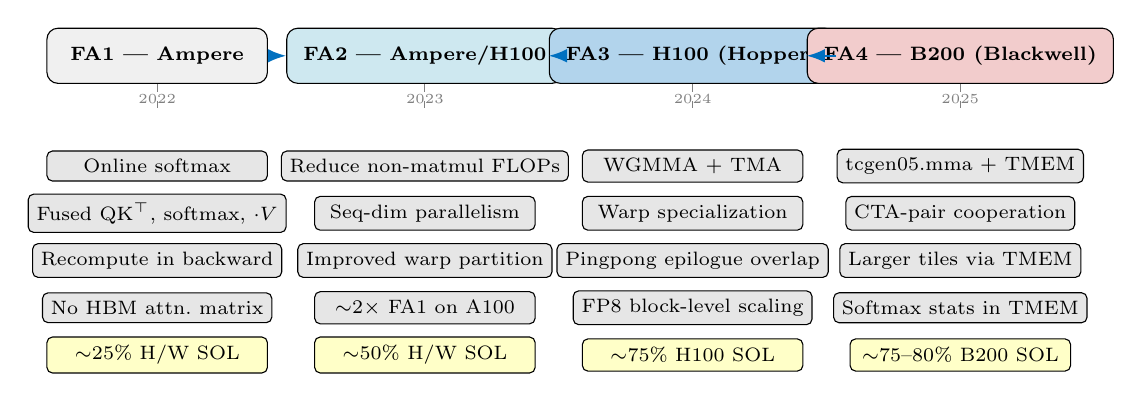
\begin{tikzpicture}[
  genbox/.style={draw, rounded corners=4pt, font=\scriptsize\bfseries, inner sep=6pt, text centered, minimum width=2.8cm, minimum height=0.7cm},
  featbox/.style={draw, rounded corners=2pt, font=\scriptsize, inner sep=3pt, text centered, minimum width=2.8cm, fill=lightgray},
  arrow/.style={-{Latex}, thick},
]
% Generation headers
\node[genbox, fill=lightgray!60] (fa1) at (0,0) {FA1 --- Ampere};
\node[genbox, fill=lightblue!60] (fa2) at (3.4,0) {FA2 --- Ampere/H100};
\node[genbox, fill=hopperblue!30] (fa3) at (6.8,0) {FA3 --- H100 (Hopper)};
\node[genbox, fill=blackwellred!20] (fa4) at (10.2,0) {FA4 --- B200 (Blackwell)};

% Year labels
\node[font=\tiny, gray] at (0,-0.55) {2022};
\node[font=\tiny, gray] at (3.4,-0.55) {2023};
\node[font=\tiny, gray] at (6.8,-0.55) {2024};
\node[font=\tiny, gray] at (10.2,-0.55) {2025};

% FA1 features
\node[featbox] (f1a) at (0,-1.4) {Online softmax};
\node[featbox] (f1b) at (0,-2.0) {Fused QK$^\top$, softmax, $\cdot V$};
\node[featbox] (f1c) at (0,-2.6) {Recompute in backward};
\node[featbox] (f1d) at (0,-3.2) {No HBM attn.\ matrix};
\node[featbox, fill=lightyellow] (f1e) at (0,-3.8) {$\sim$25\% H/W SOL};

% FA2 features
\node[featbox] (f2a) at (3.4,-1.4) {Reduce non-matmul FLOPs};
\node[featbox] (f2b) at (3.4,-2.0) {Seq-dim parallelism};
\node[featbox] (f2c) at (3.4,-2.6) {Improved warp partition};
\node[featbox] (f2d) at (3.4,-3.2) {$\sim$2$\times$ FA1 on A100};
\node[featbox, fill=lightyellow] (f2e) at (3.4,-3.8) {$\sim$50\% H/W SOL};

% FA3 features
\node[featbox] (f3a) at (6.8,-1.4) {WGMMA + TMA};
\node[featbox] (f3b) at (6.8,-2.0) {Warp specialization};
\node[featbox] (f3c) at (6.8,-2.6) {Pingpong epilogue overlap};
\node[featbox] (f3d) at (6.8,-3.2) {FP8 block-level scaling};
\node[featbox, fill=lightyellow] (f3e) at (6.8,-3.8) {$\sim$75\% H100 SOL};

% FA4 features
\node[featbox] (f4a) at (10.2,-1.4) {tcgen05.mma + TMEM};
\node[featbox] (f4b) at (10.2,-2.0) {CTA-pair cooperation};
\node[featbox] (f4c) at (10.2,-2.6) {Larger tiles via TMEM};
\node[featbox] (f4d) at (10.2,-3.2) {Softmax stats in TMEM};
\node[featbox, fill=lightyellow] (f4e) at (10.2,-3.8) {$\sim$75--80\% B200 SOL};

% Horizontal arrows between generations
\draw[arrow, hopperblue] (fa1) -- (fa2);
\draw[arrow, hopperblue] (fa2) -- (fa3);
\draw[arrow, hopperblue] (fa3) -- (fa4);

% Vertical connectors
\foreach \gen/\items in {fa1/{f1a,f1b,f1c,f1d,f1e}, fa2/{f2a,f2b,f2c,f2d,f2e}, fa3/{f3a,f3b,f3c,f3d,f3e}, fa4/{f4a,f4b,f4c,f4d,f4e}}{
  \draw[gray, dashed] (\gen.south) -- ++(0,-0.3);
}
\end{tikzpicture}
\caption{The FlashAttention lineage. Each generation targets a new NVIDIA architecture and exposes new hardware features. SOL = Speed-of-Light tensor-core throughput. Yellow cells show approximate hardware utilization achieved.}
\label{fig:fa-taxonomy}
\end{figure}

\clearpage

\subsection{FlashAttention-1: Online Softmax and IO-Awareness}
\label{sec:fa1}

The standard textbook implementation of attention computes $\mathrm{softmax}(QK^T / \sqrt{d}) V$ by materializing the $N \times N$ attention matrix $S = QK^T$ in HBM, applying softmax row-wise, and then multiplying by $V$. For sequence length $N$ and head dimension $d$, this requires $O(N^2)$ HBM writes and reads of the intermediate matrix, which dominates the total memory traffic of the operation as soon as $N \gg d$. On A100 in FP16, attention at sequence length 2048 spends roughly 80\% of its time in HBM traffic and only 20\% in tensor-core compute, despite the operation being algorithmically dominated by matmul. This was the central observation of FlashAttention-1 \citep{dao2022flashattention}: attention is memory-bound, not compute-bound, and the path to higher throughput runs through eliminating the HBM materialization of $S$ rather than through faster matmul.

\begin{figure}[t]
\centering
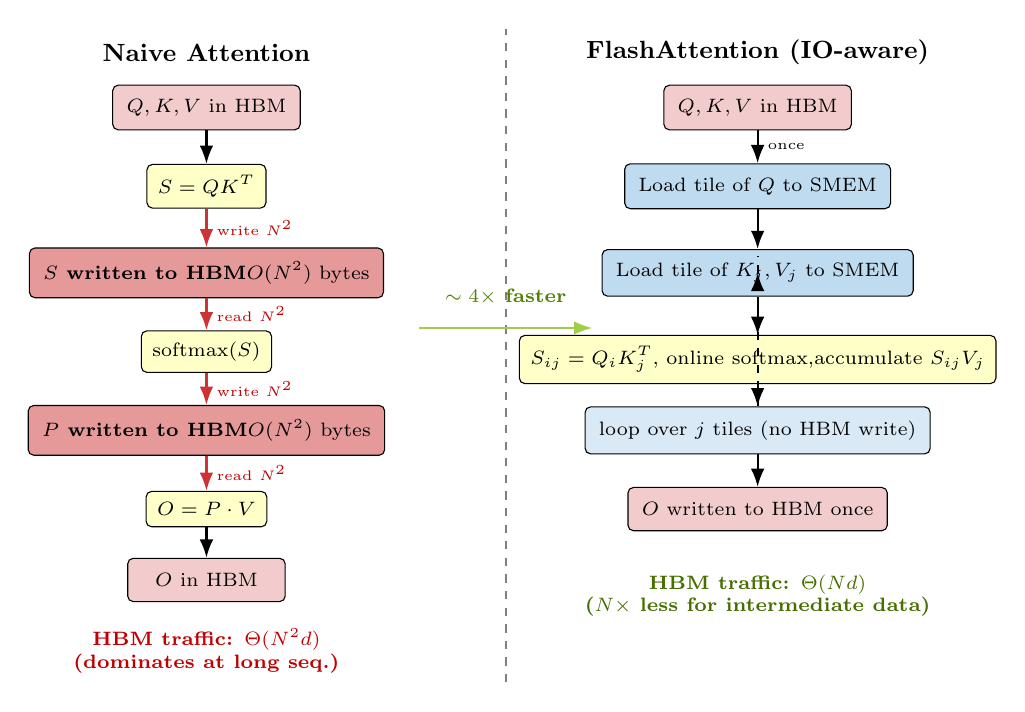
\begin{tikzpicture}[
  hbm/.style={draw, fill=blackwellred!20, rounded corners=2pt, font=\scriptsize, inner sep=5pt, minimum width=2.0cm, minimum height=0.55cm, text centered},
  smem/.style={draw, fill=hopperblue!25, rounded corners=2pt, font=\scriptsize, inner sep=5pt, minimum width=2.0cm, minimum height=0.55cm, text centered},
  op/.style={draw, fill=lightyellow, rounded corners=2pt, font=\scriptsize, inner sep=4pt, text centered},
  arr/.style={-{Latex}, thick},
  darr/.style={-{Latex}, thick, blackwellred!80},
]
% === Left side: Naive attention ===
\node[font=\small\bfseries] at (2.5, 5.5) {Naive Attention};

\node[hbm] (qkv_n) at (2.5, 4.8) {$Q, K, V$ in HBM};
\node[op] (qkt_n) at (2.5, 3.8) {$S = QK^T$};
\draw[arr] (qkv_n) -- (qkt_n);

\node[hbm, fill=blackwellred!40] (s_hbm) at (2.5, 2.7) {\textbf{$S$ written to HBM}\\$O(N^2)$ bytes};
\draw[darr] (qkt_n) -- (s_hbm) node[midway, right, font=\tiny, blackwellred] {write $N^2$};

\node[op] (sfx_n) at (2.5, 1.7) {softmax($S$)};
\draw[darr] (s_hbm) -- (sfx_n) node[midway, right, font=\tiny, blackwellred] {read $N^2$};

\node[hbm, fill=blackwellred!40] (p_hbm) at (2.5, 0.7) {\textbf{$P$ written to HBM}\\$O(N^2)$ bytes};
\draw[darr] (sfx_n) -- (p_hbm) node[midway, right, font=\tiny, blackwellred] {write $N^2$};

\node[op] (pv_n) at (2.5, -0.3) {$O = P \cdot V$};
\draw[darr] (p_hbm) -- (pv_n) node[midway, right, font=\tiny, blackwellred] {read $N^2$};

\node[hbm] (out_n) at (2.5, -1.2) {$O$ in HBM};
\draw[arr] (pv_n) -- (out_n);

% HBM traffic annotation
\node[font=\scriptsize\bfseries, blackwellred, align=center] at (2.5, -2.1) {HBM traffic: $\Theta(N^2 d)$\\(dominates at long seq.)};

% === Right side: FlashAttention ===
\node[font=\small\bfseries] at (9.5, 5.5) {FlashAttention (IO-aware)};

\node[hbm] (qkv_fa) at (9.5, 4.8) {$Q, K, V$ in HBM};
\node[smem] (qtile) at (9.5, 3.8) {Load tile of $Q$ to SMEM};
\draw[arr] (qkv_fa) -- (qtile) node[midway, right, font=\tiny] {once};

\node[smem] (kv_tile) at (9.5, 2.7) {Load tile of $K_j, V_j$ to SMEM};
\draw[arr] (qtile) -- (kv_tile);

\node[op] (fused) at (9.5, 1.6) {$S_{ij} = Q_i K_j^T$, online softmax,\\accumulate $S_{ij} V_j$};
\draw[arr] (kv_tile) -- (fused);

\node[smem, fill=hopperblue!15] (loop) at (9.5, 0.7) {loop over $j$ tiles (no HBM write)};
\draw[arr] (fused) -- (loop);
\draw[arr, dashed] (loop) |- (kv_tile);

\node[hbm] (out_fa) at (9.5, -0.3) {$O$ written to HBM once};
\draw[arr] (loop) -- (out_fa);

% HBM traffic annotation
\node[font=\scriptsize\bfseries, nvidiagreen!60!black, align=center] at (9.5, -1.4) {HBM traffic: $\Theta(Nd)$\\($N\times$ less for intermediate data)};

% Divider
\draw[gray, dashed, thick] (6.3, -2.5) -- (6.3, 5.8);

% Comparison arrow
\draw[-{Latex}, thick, nvidiagreen!70] (5.2, 2.0) -- (7.4, 2.0);
\node[font=\scriptsize\bfseries, nvidiagreen!70!black] at (6.3, 2.4) {$\sim 4\times$ faster};
\end{tikzpicture}
\caption{Comparison of naive attention (left) and FlashAttention-1 (right) in terms of HBM memory traffic. Naive attention materializes the $N\times N$ attention score matrix $S$ and probability matrix $P$ in HBM, requiring $O(N^2)$ read/write operations. FlashAttention eliminates both intermediate materializations via tile-based online softmax, reducing HBM traffic to $O(Nd)$. For $N=4096$, $d=128$, this represents a $32\times$ reduction in intermediate HBM traffic.}
\label{fig:fa-io}
\end{figure}

The technical mechanism is the well-known \emph{online softmax} algorithm \citep{milakov2018onlinesoftmax}, which computes softmax in a streaming fashion using a running maximum and a running normalizing constant. Concretely, given a sequence of input vectors processed in tiles, the online softmax tracks two scalars per row---the running max $m$ and the running denominator $\ell$---and updates them as each new tile arrives, rescaling the partial output as needed. This allows softmax to be fused with the surrounding matmuls into a single kernel: the kernel loads a tile of $Q$ once, then iterates over tiles of $K$ and $V$, computing $S_{ij} = Q_i K_j^T$, updating the online softmax statistics, and accumulating $S_{ij} V_j$ into the output, all without ever writing $S$ to HBM. The total HBM traffic drops from $O(N^2)$ to $O(N)$ for the activations, transforming attention from a memory-bound operation into one whose throughput is determined by tensor-core compute on the constituent matmuls.

A second contribution of the original FlashAttention paper is the backward-pass formulation. Naively, the backward pass requires the saved attention matrix $S$ from the forward pass, which would defeat the purpose of not materializing it. FlashAttention-1 instead recomputes $S$ tile by tile during the backward pass, paying a small additional compute cost in exchange for avoiding the HBM read. Because the forward pass is memory-bound, this tradeoff is favorable: the recomputation cost is hidden behind the memory traffic that the backward pass would do anyway. The end result is that FlashAttention-1 achieved roughly $2$--$4\times$ wallclock speedup over the standard PyTorch attention implementation on A100 across a wide range of sequence lengths, with no change in numerical results.

The impact of FlashAttention-1 went beyond the immediate speedup. By demonstrating concretely that a kernel rewrite could yield several times more end-to-end throughput than algorithmic changes (like sparse or low-rank attention) had managed, the paper shifted the field's attention toward IO-aware kernel engineering as a first-class technique for efficient deep learning. Almost every subsequent attention paper now includes a kernel-level analysis as standard practice, and the design pattern of fusing matmul with surrounding element-wise operations to avoid HBM round-trips has become ubiquitous \citep{horace2023flash}.

\subsection{FlashAttention-2: Better Work Partitioning}
\label{sec:fa2}

The FlashAttention-2 paper \citep{dao2023flashattention2} addressed two limitations of FA1 that became apparent as the technique was deployed at scale. The first was that FA1 spent more time on non-matmul operations (softmax bookkeeping, online statistics updates, output rescaling) than was strictly necessary; the second was that FA1's parallelization scheme was suboptimal on long sequences with small batch sizes, where the number of attention heads times the batch size was insufficient to saturate all SMs.

The non-matmul reduction was achieved by restructuring the inner loop to delay rescaling: rather than rescaling the partial output at every tile boundary, FA2 keeps an unnormalized accumulator and applies the normalization only at the end of the block. This trades a small amount of register pressure for a substantial reduction in the number of element-wise operations per tile, which on A100 is enough to noticeably improve throughput.

The parallelization improvement was more substantial. FA1 parallelized over batch and head dimensions but processed each row of the output sequentially within a single CTA. For long sequences with few heads, this leaves SMs idle. FA2 instead introduces parallelism over the sequence dimension itself: different CTAs are assigned different blocks of the query rows, allowing the workload to scale to fill the GPU even for long-sequence, small-batch configurations. This required a more careful work-partitioning scheme to handle the backward pass, where the gradient computation has dependencies that cross row boundaries, but the FA2 paper shows that the overheads are small. The combined effect of the non-matmul reduction and the improved parallelization was roughly a $2\times$ speedup over FA1 on A100, bringing FA2 to within striking distance of theoretical peak for attention on Ampere.

FA2 was also the first FlashAttention version to be widely adopted in production frameworks. The reference implementation, written in CUDA with templates over head dimension and precision, became the default attention backend in PyTorch, vLLM, and most serving stacks. Triton ports of FA2 also exist and are used where the slightly lower performance is acceptable in exchange for easier modification.

\subsection{FlashAttention-3: Hopper-Native Attention}
\label{sec:fa3}

When Hopper launched in 2022, simply recompiling FA2 for the new hardware left substantial performance on the table. FA2 was designed around Ampere's synchronous \texttt{mma.sync} instructions and \texttt{cp.async} bulk copies; it did not exploit Hopper's asynchronous WGMMA, did not use TMA's tile-descriptor model, did not benefit from thread-block clusters, and certainly did not use FP8. FlashAttention-3 \citep{shah2024flashattention3} is a ground-up rewrite that exploits all of these features and that has become the canonical example of a Hopper-native production kernel.

The central architectural decision in FA3 is the producer-consumer warp-specialization pattern described in Section~\ref{sec:hw-hopper}. FA3 allocates one warp group as a producer whose only role is to issue TMA loads of $K$ and $V$ tiles into a circular SMEM buffer, and two warp groups as consumers that issue WGMMAs against the buffered tiles. Synchronization between producer and consumer is mediated by \texttt{mbarrier} arrive-wait pairs. Because TMA, WGMMA, and the barrier waits are all asynchronous, the producer and consumers can run in lockstep: the producer is always one or two iterations ahead, prefetching the next tile while the consumers are computing on the current one. This is the first kernel pattern that fully decouples memory issue from compute issue on Hopper, and it is the reason FA3 reaches roughly 75\% of H100's BF16 tensor-core peak, compared to roughly 50\% for a naively-ported FA2.

A second contribution of FA3 is the introduction of \emph{pingpong scheduling}. With two consumer warp groups, FA3 can arrange the schedule so that one warp group is in its softmax-and-rescale epilogue while the other is in its WGMMA-issuing mainloop. The two warp groups alternate roles tile by tile, hiding the cost of the relatively expensive softmax operations behind the matmul throughput. This pattern generalizes beyond attention and has been adopted in several MoE kernels we discuss in Section~\ref{sec:moe}.

The third major contribution is FP8 attention with block-level scaling. Naive FP8 attention is numerically unstable because the dynamic range of $S = QK^T$ varies enormously across rows, and applying a single per-tensor scale destroys the small entries that softmax weights heavily. FA3 instead computes scales at block granularity (one scale per tile) and folds them into the WGMMA accumulation, achieving FP8 attention whose accuracy is essentially indistinguishable from FP16 attention while running at roughly $1.6\times$ the throughput. This was the first published demonstration that FP8 attention could be used in production without degrading model quality, and it has had substantial influence on FP8 inference systems for LLMs.

The Colfax Research blog series \citep{colfax2024fa3} provides an extensive technical deep-dive on FA3, walking through the producer-consumer kernel structure, the pingpong scheduling, and the FP8 numerics in considerable detail. Together with the FA3 paper itself, these resources have become standard reading for anyone writing high-performance Hopper kernels.

\subsection{FlashAttention-4: Blackwell-Native Attention}
\label{sec:fa4}

FlashAttention-4 \citep{flashattention4} extends the lineage to Blackwell. The core algorithmic structure is unchanged---online softmax, tiled $QK^T$, fused $\cdot V$, recomputation in the backward pass---but the kernel realization is restructured around Blackwell's tcgen05 tensor cores and TMEM accumulator. The most consequential change is that the matmul accumulator now lives in TMEM rather than registers. On Hopper this constraint had limited tile sizes: a WGMMA accumulator for a $128 \times 256$ output tile in FP32 consumes 32 KB of register space per warp group, leaving little room for the rest of the kernel. Moving the accumulator to TMEM frees the register file for other uses and allows FA4 to use larger tile shapes than were practical on Hopper.

A second change is the use of CTA pairs. FA4 issues some of its tcgen05 instructions as cooperative pair operations, in which two CTAs share a single matmul instruction with operands sourced from one CTA's SMEM and accumulator stored in the other's TMEM. This effectively doubles the SMEM available to a single matmul, which is particularly useful for the long-sequence configurations where attention's working set is largest.

A third change concerns where the softmax statistics live. On Hopper, FA3 kept the running max and denominator in registers, alongside the matmul accumulator. On Blackwell, FA4 moves these statistics to TMEM as well, exploiting the fact that TMEM has dedicated load/store instructions that can update small per-row values efficiently. This restructuring required some care because the softmax update logic must be expressible in terms of TMEM operations rather than ordinary register arithmetic, but the result is a kernel whose register pressure is dramatically lower than FA3's.

Early benchmarks reported in the FA4 documentation suggest that the kernel achieves a similar fraction of B200's tensor-core peak (around 75--80\%) as FA3 did on H100, which translates into roughly $2\times$ end-to-end attention throughput improvement from H100 to B200 in BF16 and substantially more in FP4. As with FA3, the FA4 codebase is expected to become the foundation for Blackwell-native attention in vLLM, SGLang, TensorRT-LLM, and the major training frameworks.

\subsection{Generation Comparison}
\label{sec:fa-comparison}

Table~\ref{tab:fa-comparison} summarizes the four generations along the dimensions that matter for kernel writers: target hardware, the new hardware features each version exploited, the parallelization scheme, the achievable fraction of tensor-core peak, and notable software-engineering concerns.

\begin{table}[H]
\caption{FlashAttention generations and their key technical characteristics. SOL fractions are approximate and depend on shape, precision, and head count.}
\label{tab:fa-comparison}
\centering\small
\begin{tabular}{lccccc}
\toprule
Version & Target & Compute primitive & Async copy & Precision & \% SOL \\
\midrule
FA1 & A100 & mma.sync & cp.async & FP16/BF16 & $\sim 25\%$ \\
FA2 & A100/H100 & mma.sync & cp.async & FP16/BF16 & $\sim 50\%$ \\
FA3 & H100 & WGMMA (async) & TMA & FP16/BF16/FP8 & $\sim 75\%$ \\
FA4 & B200 & tcgen05.mma & TMA & FP16/BF16/FP8/FP4 & $\sim 75$--$80\%$ \\
\bottomrule
\end{tabular}
\end{table}

The pattern in Table~\ref{tab:fa-comparison} is clear: each generation captures the new hardware features of its target architecture and translates them into roughly a doubling of effective tensor-core utilization. The lineage also illustrates that high-performance kernels are not portable across architectures in any deep sense---FA2 runs correctly on Hopper but reaches only 50\% of the throughput that the Hopper-native FA3 achieves---and that the transition cost from one generation to the next is substantial. This portability problem recurs throughout the MoE kernel literature surveyed in the next section.

\section{Mixture-of-Experts Systems}
\label{sec:moe}

Mixture-of-Experts is the dominant architecture for scaling LLMs beyond the limits of dense compute. By replacing each dense feed-forward block with a set of expert blocks and routing each token to a small subset of them, MoE decouples model capacity (total parameter count) from per-token compute. The technique was popularized in its modern form by the sparsely-gated MoE paper \citep{shazeer2017outrageously} and scaled in GShard \citep{lepikhin2021gshard}, Switch Transformer \citep{fedus2022switch}, and GLaM \citep{du2022glam}; current open-weight MoE LLMs include Mixtral \citep{jiang2024mixtral}, DeepSeek-MoE \citep{dai2024deepseekmoe}, DeepSeek-V3 \citep{liu2024deepseekv3}, and Qwen-MoE. This section surveys MoE from the kernel-engineering perspective: how routing is computed, how the per-expert grouped GEMMs are mapped onto GPU tensor cores, how all-to-all communication is overlapped with compute in distributed settings, and how end-to-end MoE systems combine these techniques. Figure~\ref{fig:moe-taxonomy} organizes the literature into a taxonomy.

\begin{figure}[t]
\centering
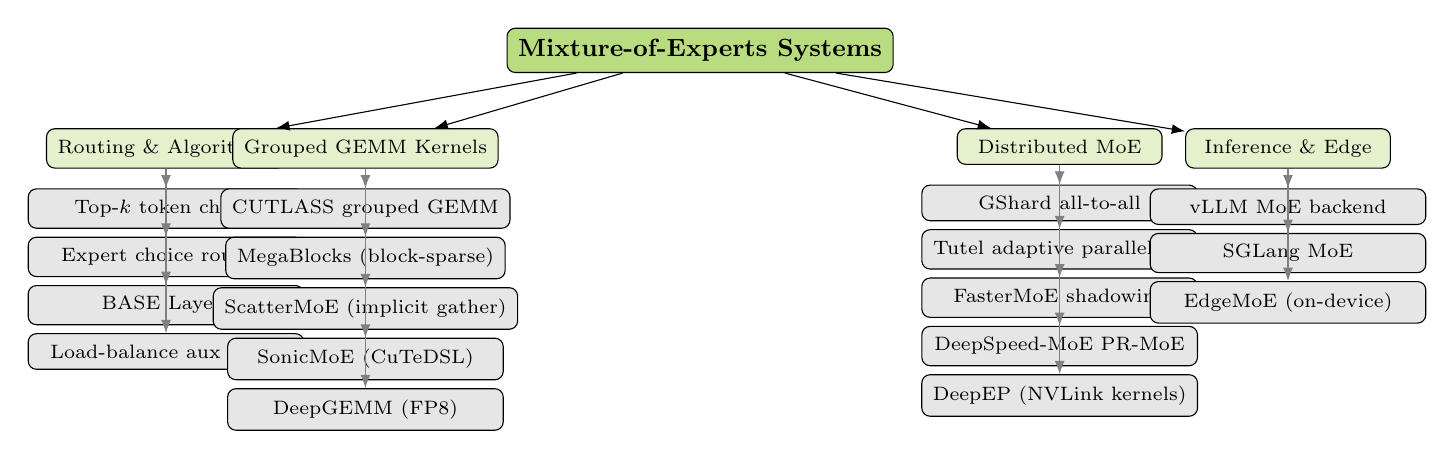
\begin{tikzpicture}[
  node distance=0.3cm and 0.4cm,
  box/.style={draw, rounded corners=3pt, font=\scriptsize, inner sep=4pt, text centered, minimum width=3.5cm},
  catbox/.style={box, fill=nvidiagreen!20, minimum width=2.6cm},
  itembox/.style={box, fill=lightgray, minimum width=3.5cm},
  rootbox/.style={box, fill=nvidiagreen!50, font=\small\bfseries, minimum width=3.4cm},
]
\node[rootbox] (root) {Mixture-of-Experts Systems};

\node[catbox, below left=0.7cm and 2.8cm of root] (route) {Routing \& Algorithms};
\node[catbox, below left=0.7cm and 0.1cm of root] (gemm) {Grouped GEMM Kernels};
\node[catbox, below right=0.7cm and 0.8cm of root] (dist) {Distributed MoE};
\node[catbox, below right=0.7cm and 3.7cm of root] (inf) {Inference \& Edge};

\node[itembox, below=0.25cm of route] (ro1) {Top-$k$ token choice};
\node[itembox, below=0.1cm of ro1] (ro2) {Expert choice routing};
\node[itembox, below=0.1cm of ro2] (ro3) {BASE Layers};
\node[itembox, below=0.1cm of ro3] (ro4) {Load-balance aux losses};

\node[itembox, below=0.25cm of gemm] (ge1) {CUTLASS grouped GEMM};
\node[itembox, below=0.1cm of ge1] (ge2) {MegaBlocks (block-sparse)};
\node[itembox, below=0.1cm of ge2] (ge3) {ScatterMoE (implicit gather)};
\node[itembox, below=0.1cm of ge3] (ge4) {SonicMoE (CuTeDSL)};
\node[itembox, below=0.1cm of ge4] (ge5) {DeepGEMM (FP8)};

\node[itembox, below=0.25cm of dist] (di1) {GShard all-to-all};
\node[itembox, below=0.1cm of di1] (di2) {Tutel adaptive parallelism};
\node[itembox, below=0.1cm of di2] (di3) {FasterMoE shadowing};
\node[itembox, below=0.1cm of di3] (di4) {DeepSpeed-MoE PR-MoE};
\node[itembox, below=0.1cm of di4] (di5) {DeepEP (NVLink kernels)};

\node[itembox, below=0.25cm of inf] (in1) {vLLM MoE backend};
\node[itembox, below=0.1cm of in1] (in2) {SGLang MoE};
\node[itembox, below=0.1cm of in2] (in3) {EdgeMoE (on-device)};

\draw[-{Latex}] (root) -- (route);
\draw[-{Latex}] (root) -- (gemm);
\draw[-{Latex}] (root) -- (dist);
\draw[-{Latex}] (root) -- (inf);

\foreach \cat/\items in {route/{ro1,ro2,ro3,ro4}, gemm/{ge1,ge2,ge3,ge4,ge5}, dist/{di1,di2,di3,di4,di5}, inf/{in1,in2,in3}}{
  \foreach \item in \items {
    \draw[-{Latex}, gray] (\cat) -- (\item);
  }
}
\end{tikzpicture}
\caption{Taxonomy of Mixture-of-Experts systems, organized by the aspect of the MoE pipeline each primarily addresses.}
\label{fig:moe-taxonomy}
\end{figure}

\subsection{MoE Background and Routing}
\label{sec:moe-background}

A standard MoE layer replaces the dense feed-forward block in a Transformer with $E$ expert feed-forward blocks and a router that, given an input token's hidden state, produces a probability distribution over experts and selects the top $k$ experts (typically $k \in \{1, 2\}$). Each token is then processed by its selected experts, and the per-expert outputs are combined via a weighted sum using the router probabilities. The total parameter count grows linearly with $E$, but the per-token compute grows only with $k$, which is what makes MoE attractive for scaling.

\begin{figure}[t]
\centering
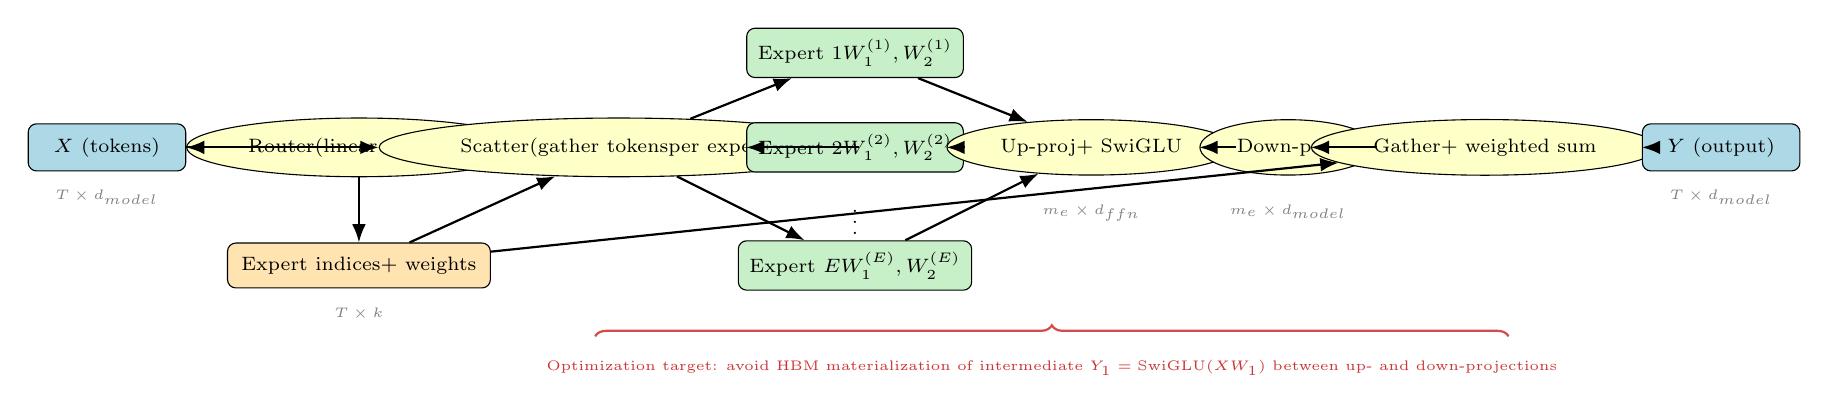
\begin{tikzpicture}[
  tensor/.style={draw, rounded corners=3pt, fill=lightblue, font=\scriptsize, inner sep=5pt, minimum width=2.0cm, minimum height=0.55cm, text centered},
  op/.style={draw, ellipse, fill=lightyellow, font=\scriptsize, inner sep=4pt, text centered},
  expert/.style={draw, rounded corners=3pt, fill=lightgreen, font=\scriptsize, inner sep=4pt, minimum width=1.6cm, minimum height=0.5cm, text centered},
  arr/.style={-{Latex}, thick},
  shape label/.style={font=\tiny, gray, anchor=north},
]
% Input
\node[tensor] (X) at (0,0) {$X$ (tokens)};
\node[shape label] at (0,-0.42) {$T \times d_\text{model}$};

% Router
\node[op] (router) at (3.2,0) {Router\\(linear + top-$k$)};
\draw[arr] (X) -- (router);

% Routing weights and indices
\node[tensor, fill=ambercolor!30] (idx) at (3.2,-1.5) {Expert indices\\+ weights};
\node[shape label] at (3.2,-1.92) {$T \times k$};
\draw[arr] (router) -- (idx);

% Scatter / gather
\node[op] (scatter) at (6.5,0) {Scatter\\(gather tokens\\per expert)};
\draw[arr] (X) -- (scatter);
\draw[arr] (idx) -- (scatter);

% Expert groups
\node[expert] (e1) at (9.5, 1.2) {Expert 1\\$W_1^{(1)}, W_2^{(1)}$};
\node[expert] (e2) at (9.5, 0.0) {Expert 2\\$W_1^{(2)}, W_2^{(2)}$};
\node[font=\scriptsize] (edots) at (9.5, -0.85) {$\vdots$};
\node[expert] (eE) at (9.5, -1.5) {Expert $E$\\$W_1^{(E)}, W_2^{(E)}$};

\draw[arr] (scatter) -- (e1);
\draw[arr] (scatter) -- (e2);
\draw[arr] (scatter) -- (eE);

% Per expert: up-proj -> activation -> down-proj
\node[op] (up) at (12.5, 0.0) {Up-proj\\$+$ SwiGLU};
\draw[arr] (e1) -- (up);
\draw[arr] (e2) -- (up);
\draw[arr] (eE) -- (up);
\node[shape label] at (12.5,-0.6) {$m_e \times d_\text{ffn}$};

\node[op] (down) at (15.0, 0.0) {Down-proj};
\draw[arr] (up) -- (down);
\node[shape label] at (15.0,-0.6) {$m_e \times d_\text{model}$};

% Gather + weighted sum
\node[op] (gather) at (17.5, 0.0) {Gather\\+ weighted sum};
\draw[arr] (down) -- (gather);
\draw[arr] (idx) -- (gather);

% Output
\node[tensor] (Y) at (20.5, 0.0) {$Y$ (output)};
\node[shape label] at (20.5,-0.42) {$T \times d_\text{model}$};
\draw[arr] (gather) -- (Y);

% Annotation: HBM round trips
\draw[decorate, decoration={brace, amplitude=4pt}, thick, blackwellred!70]
  (6.2, -2.4) -- (17.8, -2.4)
  node[midway, below=5pt, font=\tiny, blackwellred!80, align=center] {Optimization target: avoid HBM materialization of intermediate $Y_1 = \mathrm{SwiGLU}(X W_1)$ between up- and down-projections};
\end{tikzpicture}
\caption{Data flow through an MoE layer. Input tokens are scored by the router; each token is scattered to its top-$k$ assigned experts. Each expert independently computes an up-projection followed by SwiGLU and a down-projection. Expert outputs are gathered and combined with router weights. The intermediate activation $Y_1$ between the two GEMMs is the primary fusion target: materializing it in HBM and reading it back costs $O(T \cdot d_\text{ffn})$ bytes of unnecessary HBM traffic per layer.}
\label{fig:moe-dataflow}
\end{figure}

The router itself is a small linear projection followed by a softmax and a top-$k$ selection. The dominant routing strategy, introduced by \citet{shazeer2017outrageously} and refined by Switch Transformer \citep{fedus2022switch}, is \emph{token choice}: each token independently selects its top $k$ experts. Token choice has the property that the per-expert load is unbalanced---some experts receive far more tokens than others on a given batch---which creates a kernel-level problem (irregular per-expert matmul shapes) and a system-level problem (some experts oversaturate while others sit idle). Switch Transformer addressed the imbalance with an auxiliary load-balancing loss that encourages the router to spread tokens evenly across experts, and with a \emph{capacity factor} that caps the number of tokens any single expert can receive (excess tokens are dropped). The capacity-and-drop approach trades a small amount of model quality for predictable kernel shapes.

Two alternative routing strategies eliminate token dropping at the cost of more complex routing logic. \emph{Expert choice} \citep{zhou2022expertchoice} inverts the assignment: each expert selects its top-$k$ tokens rather than each token selecting its top-$k$ experts. This guarantees perfect per-expert load balance and eliminates dropping entirely, but it changes the semantics of the model (a token may be processed by zero, one, or many experts). \emph{BASE Layers} \citep{lewis2021base} formulate routing as a linear assignment problem solved via the auction algorithm, achieving exact load balance with token-choice-like semantics. StableMoE \citep{dai2022stablemoe} addresses a different problem: routing instability during training, in which the same token is routed to different experts at different training steps because the router weights are still moving. StableMoE distills a stable router from a converged routing strategy, freezing the assignments early in training. X-MoE \citep{chi2022xmoe} addresses representation collapse, in which the experts learn nearly identical functions, by routing on a low-dimensional hypersphere.

For the purposes of this survey, the most important consequence of these routing variants is that they all produce, downstream, a sequence of grouped GEMMs whose shapes vary at runtime. The remaining MoE kernel work---grouped GEMM implementations, fusion patterns, distributed communication---is essentially independent of which routing strategy is used and can be applied uniformly. We therefore turn to grouped GEMM as the central kernel-level problem.

\subsection{Grouped GEMM Implementations}
\label{sec:moe-groupedgemm}

The forward pass of an MoE layer reduces, after routing, to a sequence of independent matrix multiplications, one per expert. If expert $e$ receives $m_e$ tokens, then the up-projection for expert $e$ is a matmul of shape $(m_e \times d_{\text{model}}) \cdot (d_{\text{model}} \times d_{\text{ffn}})$, and similarly for the down-projection. The set of all per-expert matmuls is what is conventionally called a \emph{grouped GEMM}. Three properties make grouped GEMM hard to implement efficiently. First, the per-group $M$ dimensions $m_e$ vary at runtime and may differ by an order of magnitude across experts in the same batch. Second, the total work is small enough that launching $E$ separate GEMM kernels (one per expert) incurs prohibitive launch overhead. Third, the expert weights $W_e$ must be staged from HBM, and naive implementations end up reading the same weight tile multiple times if the SM scheduling does not cooperate with the weight layout.

\paragraph{CUTLASS Grouped GEMM.}
NVIDIA's CUTLASS library has provided a templated grouped GEMM implementation since version 2.x \citep{thakkar2023cutlass}. The CUTLASS grouped GEMM kernel takes a list of per-group problem sizes and pointers and dispatches all groups in a single kernel launch, eliminating the launch-overhead problem. Each CTA processes one tile from one group, and a global work-stealing scheduler distributes tiles across SMs. CUTLASS grouped GEMM is the baseline against which most MoE-specific kernels are compared, and it remains the highest-performing general-purpose grouped GEMM available for NVIDIA hardware. Its main limitation for MoE is that it does not exploit the structural properties of the MoE problem---in particular, that all groups share the same $K$ and $N$ dimensions and only the $M$ dimension varies---and so leaves some L2-locality and instruction-scheduling optimizations on the table.

\paragraph{MegaBlocks.}
MegaBlocks \citep{gale2023megablocks}, developed at Stanford and Databricks, takes a fundamentally different approach. Rather than treating MoE as a sequence of independent matmuls, MegaBlocks reformulates the MoE forward pass as a single block-sparse matmul: the input is the concatenated stack of all tokens, the weight is a block-diagonal matrix with one block per expert, and the output is the concatenated stack of expert outputs. Block-sparsity captures the routing structure exactly---each token interacts only with its assigned experts---and the resulting matmul can be implemented as a custom block-sparse GEMM kernel that processes only the non-zero blocks. The MegaBlocks paper introduces hand-tuned block-sparse GPU kernels that outperform CUTLASS grouped GEMM by 30--60\% on typical MoE shapes. Equally important, the block-sparse formulation is naturally drop-free: there is no capacity factor and no token dropping, because the kernel processes whatever routing assignment the router produces. This both improves model quality (no information loss from dropped tokens) and simplifies the training pipeline (no capacity tuning). MegaBlocks has become the reference implementation for high-performance MoE training and is integrated into Megatron, Composer, and Nanotron.

\paragraph{ScatterMoE.}
ScatterMoE \citep{tan2024scattermoe} is a more recent grouped GEMM implementation that focuses on minimizing intermediate buffer materialization. The key observation is that conventional grouped GEMM implementations physically gather tokens into per-expert buffers before the matmul (so that expert $e$'s input is a contiguous $m_e \times d$ matrix) and then physically scatter the outputs back. These gather and scatter operations cost HBM bandwidth and create memory-allocation pressure. ScatterMoE instead performs the gather and scatter \emph{implicitly}, inside the matmul kernel, by indexing into the unsorted token buffer using pre-computed gather indices. The result is a grouped GEMM with no intermediate buffer materialization and roughly 30\% lower HBM traffic than MegaBlocks on typical configurations. ScatterMoE is used as the default MoE backend in several training frameworks.

\paragraph{SonicMoE.}
SonicMoE \citep{sonicmoe2025} pushes the optimization further by writing Hopper-native CuTeDSL kernels that exploit WGMMA, TMA, and warp specialization in the same way FlashAttention-3 does for attention. The SonicMoE up-projection kernel fuses gather, $X \cdot W_1$, and SwiGLU into a single producer-consumer kernel; the down-projection kernel fuses $Y_1 \cdot W_2$ and the expert-weighted scatter-sum. Each kernel is roughly 3000 lines of CuTeDSL and uses persistent CTAs with L2-aware rasterization to maximize weight reuse across the tiles assigned to each SM. The reported speedup is $1.86\times$ over ScatterMoE on H100 with a 45\% reduction in activation memory. SonicMoE represents the current state of the art for single-node MoE training kernels on Hopper and serves as the case study for the L2/SMEM fusion techniques discussed in Section~\ref{sec:fusion}.

\paragraph{DeepGEMM and DeepEP.}
DeepGEMM \citep{deepgemm2024} is DeepSeek's open-source FP8 GEMM library, originally developed for DeepSeek-V3 training. It includes both standard and grouped GEMM kernels and is notable for its aggressive use of FP8 with fine-grained per-block scaling, achieving FP8 throughput close to the hardware peak on H800 GPUs (a Hopper variant). DeepEP \citep{deepep2024}, also from DeepSeek, is a companion library that provides high-performance all-to-all communication kernels for distributed MoE; we discuss it in Section~\ref{sec:moe-distributed}.

\subsection{Distributed MoE Systems}
\label{sec:moe-distributed}

For models with hundreds of experts or trillions of total parameters, the experts cannot all fit on a single GPU and must be sharded across devices. Expert parallelism, introduced in GShard \citep{lepikhin2021gshard}, places different experts on different GPUs and uses an all-to-all communication step to move tokens from their home device to the device hosting their assigned expert (and another all-to-all to move outputs back). The all-to-all is the dominant communication cost in distributed MoE training, and the engineering of this step has been the subject of an extensive literature.

\paragraph{FastMoE and FasterMoE.}
FastMoE \citep{he2021fastmoe} was the first widely-used distributed MoE training system, providing PyTorch-integrated all-to-all primitives and a hierarchical interface compatible with Megatron-LM and Transformer-XL. FasterMoE \citep{he2022fastermoe} extends FastMoE with three optimizations: a roofline-based performance model that predicts all-to-all latency, a dynamic shadowing technique that replicates hot experts across devices to reduce load imbalance, and a fine-grained schedule that overlaps the all-to-all with the local expert compute. The reported speedups range from $1.4\times$ to nearly $18\times$ over baseline implementations like ZeRO and GShard.

\paragraph{Tutel.}
Tutel \citep{hwang2023tutel}, developed at Microsoft, focuses on adapting MoE parallelism to dynamic workloads. The central observation is that the optimal parallelism strategy (data parallel vs.\ expert parallel vs.\ tensor parallel mixes) depends on the per-expert token counts, which vary batch to batch. Tutel implements a switchable parallelism layer that can transition between strategies at runtime without tensor migration costs, and it supports adaptive pipelining that reshapes the all-to-all schedule based on the current load distribution. Tutel reports up to $5.75\times$ speedup over baseline expert-parallel implementations on a single MoE layer.

\paragraph{DeepSpeed-MoE.}
DeepSpeed-MoE \citep{rajbhandari2022deepspeedmoe}, from Microsoft Research, contributes both a new MoE architecture (Pyramid-Residual MoE, which combines dense and sparse layers in a hybrid structure) and a highly-optimized inference engine. The PR-MoE design reduces total parameter count by up to $3\times$ without sacrificing quality, while the inference engine delivers up to $7.3\times$ lower latency and $9\times$ lower cost than quality-equivalent dense models. DeepSpeed-MoE has been used to serve some of the largest production MoE models and remains a reference point for MoE inference systems.

\paragraph{Topology-Aware and Auto-Parallel MoE.}
TA-MoE \citep{chen2022tamoe} observes that conventional MoE dispatch patterns ignore the heterogeneous bandwidth structure of modern GPU clusters (intra-node NVLink vs.\ inter-node InfiniBand) and proposes a topology-aware routing strategy that biases token assignments toward experts on nearby devices. Lina \citep{li2023lina} similarly prioritizes all-to-all over allreduce in training and balances workloads dynamically in inference. SmartMoE \citep{zhai2023smartmoe} automates the parallelization choice itself: in an offline phase, SmartMoE constructs a search space of hybrid parallelism strategies, and at runtime it picks the best strategy for the current input distribution. The reported gains range from 1.4$\times$ to nearly 2$\times$ over hand-tuned FasterMoE configurations.

\paragraph{DeepEP.}
DeepEP \citep{deepep2024} is the most recent significant contribution to distributed MoE communication. Released as part of the DeepSeek open-source initiative, DeepEP provides hand-optimized all-to-all kernels written directly in PTX with careful overlap of NVLink and InfiniBand traffic. The library achieves close to peak NVLink bandwidth on intra-node all-to-all and substantially improves inter-node all-to-all over baseline NCCL. DeepEP is now the default communication backend for DeepSeek-V3 training and has been adopted in several other large-scale MoE projects.

\subsection{Inference, Edge, and Smaller-Scale MoE}
\label{sec:moe-inference}

MoE inference has its own kernel-level concerns. The primary one is that, at inference time, batch sizes are often small (especially for latency-sensitive serving), which exacerbates the per-expert $M$-dimension problem: with a batch size of 1 and top-$k$ of 2, each token visits 2 experts and each visited expert sees a single token. The grouped GEMM degenerates into a sequence of skinny matmuls that are essentially purely memory-bound, and most of the optimization targets the HBM traffic of the expert weights themselves rather than the matmul compute.

\paragraph{vLLM and SGLang.}
The major LLM serving frameworks have all added MoE support. vLLM \citep{kwon2023vllm} supports Mixtral, DeepSeek-MoE, and other open-weight MoE models via a backend that reuses the framework's PagedAttention infrastructure for KV-cache management and adds custom grouped GEMM kernels for the expert layers. SGLang \citep{zheng2024sglang} provides similar support with additional structured-output optimizations. Both frameworks rely on FlashAttention-3 for attention and on either CUTLASS grouped GEMM or custom Triton kernels for the expert layers.

\paragraph{EdgeMoE.}
EdgeMoE \citep{yi2023edgemoe} addresses the opposite extreme: serving MoE models on a single edge device where total expert weights exceed device memory. The system stores non-expert weights in device memory and keeps expert weights on external storage (SSD or eMMC), loading individual experts on demand when their tokens arrive. The challenge is to overlap the SSD-to-DRAM-to-GPU expert transfer with the compute on already-resident experts. EdgeMoE reports practical inference of moderate-size MoE models on mobile-class hardware, opening an interesting design space for on-device MoE.

\subsection{System Comparison}
\label{sec:moe-comparison}

Table~\ref{tab:moe-systems} summarizes the main MoE systems along the dimensions of grouped GEMM strategy, distributed communication strategy, target hardware, and supported precision. The pattern is that single-node optimization (better grouped GEMM kernels) and distributed-node optimization (better all-to-all and parallelism strategies) have largely been pursued independently, with most systems specializing in one or the other. SonicMoE's contribution is a particularly aggressive single-node optimization on Hopper; DeepEP's is a corresponding aggressive distributed-node optimization. A fully optimized end-to-end MoE training system today combines a SonicMoE-class single-node kernel stack with a DeepEP-class communication stack, plus a Tutel- or SmartMoE-class adaptive parallelism layer on top.

\begin{table}[t]
\caption{Comparison of major MoE systems, organized by the layer of the stack each primarily addresses.}
\label{tab:moe-systems}
\centering\small
\begin{tabular}{lccc}
\toprule
System & Primary contribution & Target & Drop-free? \\
\midrule
GShard \citep{lepikhin2021gshard} & Distributed expert parallelism & TPU/GPU & no \\
Switch Transformer \citep{fedus2022switch} & Top-1 routing + load balancing & TPU/GPU & no \\
FastMoE \citep{he2021fastmoe} & PyTorch all-to-all primitives & GPU & no \\
FasterMoE \citep{he2022fastermoe} & Shadowing + roofline scheduling & GPU & no \\
Tutel \citep{hwang2023tutel} & Adaptive parallelism + pipelining & GPU & no \\
DeepSpeed-MoE \citep{rajbhandari2022deepspeedmoe} & PR-MoE + inference engine & GPU & no \\
MegaBlocks \citep{gale2023megablocks} & Block-sparse GEMM kernels & A100/H100 & yes \\
ScatterMoE \citep{tan2024scattermoe} & Implicit scatter/gather GEMM & A100/H100 & yes \\
SonicMoE \citep{sonicmoe2025} & CuTeDSL Hopper-native kernels & H100 & yes \\
DeepGEMM \citep{deepgemm2024} & FP8 grouped GEMM & H800/H100 & yes \\
DeepEP \citep{deepep2024} & Hand-tuned all-to-all kernels & H800/H100 & yes \\
EdgeMoE \citep{yi2023edgemoe} & On-device MoE serving & Edge/mobile & N/A \\
\bottomrule
\end{tabular}
\end{table}

The pattern in Table~\ref{tab:moe-systems} also reflects a generational shift: pre-2023 systems focused almost exclusively on the distributed communication problem (because grouped GEMM was assumed to be a solved problem handled by CUTLASS), while post-2023 systems---MegaBlocks, ScatterMoE, SonicMoE, DeepGEMM---increasingly recognized that the single-node grouped GEMM was leaving substantial performance on the table on Hopper-class hardware. The frontier today is the integration of these two streams: single-node kernels written in CuTeDSL or ThunderKittens, combined with hand-tuned all-to-all kernels in the style of DeepEP, deployed in adaptive parallelism frameworks like SmartMoE. The case study in Section~\ref{sec:fusion} examines how the L2 and SMEM levels of the memory hierarchy can be exploited at the seams between these two streams.

% =====================================================================
% New bibliography entries introduced in Pass 2
% Append to the main thebibliography in moe_gpu_survey.tex
% (Most other keys used here already exist from the initial draft.)
% =====================================================================

% \bibitem{milakov2018onlinesoftmax} Milakov, M., Gimelshein, N. Online normalizer calculation for softmax. \emph{arXiv:1805.02867}, 2018.
\bibitem{rouhani2023microscaling} Rouhani, B.~D., et al. Microscaling data formats for deep learning. \emph{arXiv:2310.10537}, 2023.
\bibitem{williams2009roofline} Williams, S., Waterman, A., Patterson, D. Roofline: an insightful visual performance model for multicore architectures. \emph{Communications of the ACM}, 52(4):65--76, 2009.
\bibitem{luo2024hopperdissect} Luo, W., Fan, R., Li, Z., Du, D., Wang, Q., Chu, X. Benchmarking and dissecting the NVIDIA Hopper GPU architecture. \emph{arXiv:2402.13499}, 2024.
% =====================================================================
% PASS 3: Sections 6, 7, 8, 9 — drop-in replacement for the existing
% short versions of these sections in main.tex.
% Same packages required (booktabs, tikz, forest).
% =====================================================================

\section{Memory Hierarchy Optimizations and Kernel Fusion}
\label{sec:fusion}

The previous sections traced two largely independent threads of work: matmul kernel engineering (Section~\ref{sec:matmul}) and MoE-specific systems (Section~\ref{sec:moe}). This section addresses the techniques that live at the seams between kernels---the fusion patterns that determine how data flows between consecutive operations and how aggressively the memory hierarchy is exploited. On Hopper and Blackwell, with their large L2 caches and abundant SMEM, fusion is increasingly the dominant lever for end-to-end MoE throughput once the constituent kernels are individually well tuned. We organize the discussion around a cost model for data movement, then survey the major fusion patterns, and conclude with a worked case study of L2-cache-warm and SMEM-level fusion applied to an MoE forward pass.

\subsection{A Cost Model for Data Movement}
\label{sec:fusion-costmodel}

Every byte of data accessed by a kernel lives at exactly one level of the memory hierarchy at any moment, and moving it between levels has a quantifiable cost. On H100, a byte read from registers is effectively free (one clock, no contention); a byte read from SMEM costs roughly $5\times$ more bandwidth-wise than a register read; a byte read from L2 costs roughly $1.6\times$ more than an SMEM read; and a byte read from HBM costs roughly $3.6\times$ more than an L2 read. The compounding factor from registers to HBM is therefore roughly $30\times$. This is the cost model that the rest of this section operates under.

The implication for kernel fusion is direct. If two consecutive kernels share a tensor $T$ of size $|T|$ bytes, then materializing $T$ in HBM (the default behavior of two separately-launched kernels) costs $2 \cdot |T|$ bytes of HBM traffic (one write by the producer, one read by the consumer). If the kernels can be arranged so that $T$ is read from L2 instead, the cost drops by roughly $3.6\times$ on the read side; if from SMEM, by roughly another $1.6\times$; if $T$ never leaves registers, the cost approaches zero. The end-to-end speedup that any given fusion delivers can be computed by adding up the bytes saved across the levels of the hierarchy and dividing by the total memory traffic of the unfused baseline. For MoE intermediate activations of tens of megabytes per layer, fusion gains in the low single digits per layer compound to substantial end-to-end speedups across the 32--64 layers of a typical model.

\subsection{Fusion Patterns}
\label{sec:fusion-patterns}

We distinguish four broad categories of fusion that recur in the MoE literature.

\paragraph{Vertical fusion (operator + epilogue).}
The simplest and most widely-used fusion pattern combines a GEMM with the element-wise operation that follows it: GEMM~+~bias, GEMM~+~activation, GEMM~+~SwiGLU, GEMM~+~quantize. The element-wise op runs on the matmul accumulator while it is still in registers, before the result is written to SMEM or HBM. CUTLASS supports this pattern via its epilogue functor template parameter, and CUTLASS 3.x's epilogue visitor pattern generalizes it to chains of element-wise operations. Vertical fusion is essentially mandatory for high performance: a GEMM followed by a separate element-wise kernel pays an extra HBM round trip for no algorithmic benefit, and modern libraries make the fused version no harder to write.

\paragraph{Horizontal fusion (parallel ops sharing inputs).}
Horizontal fusion combines independent operations that read the same input tensor into a single kernel that reads the input once. The canonical example in Transformers is the Q/K/V projection: three separate linear layers that all read the same hidden state and could share the load. Horizontal fusion is more situational than vertical fusion---it requires that the parallel ops have similar shapes and computation costs---but where it applies, it eliminates redundant HBM traffic.

\paragraph{Cross-layer fusion (megakernels).}
Cross-layer fusion combines two or more logically distinct operations into a single kernel that processes them sequentially while keeping intermediate data in fast memory. The MoE forward pass is the prototypical target: the up-projection produces an intermediate tensor that the down-projection consumes, and a cross-layer fusion can keep this intermediate in L2 or even SMEM rather than spilling it to HBM. Cross-layer fusion is harder to implement than vertical or horizontal fusion because the two operations may have different optimal tile shapes, different SMEM budgets, and different scheduling constraints. The reward, when it works, is the elimination of an entire round trip to HBM for the intermediate tensor.

\paragraph{Persistent kernels.}
Persistent kernels occupy a slightly orthogonal axis. Rather than launching one CTA per output tile, a persistent kernel launches exactly enough CTAs to fill the GPU and has each CTA process multiple tiles in sequence, pulling work from a global queue. The benefits are reduced launch overhead, better L2 locality (because consecutive tiles processed by the same CTA can share L2-resident weight tiles), and the ability to coordinate cross-tile scheduling. Persistent kernels are now standard in CUTLASS 3.x and in most Hopper-native FlashAttention and grouped GEMM implementations \citep{shah2024flashattention3,thakkar2023cutlass}. The cudaforfun ``Outperforming cuBLAS'' worklog \citep{cudaforfun2024} provides a detailed walkthrough of how persistent CTAs combined with L2-aware rasterization can extract several percent of additional performance over a non-persistent baseline.

These four patterns are not mutually exclusive. A modern Hopper MoE kernel typically uses vertical fusion (GEMM + SwiGLU), persistent CTAs with L2 rasterization, and cross-layer fusion of the up- and down-projections, all in the same implementation. The case study below works through such an integrated example in detail.

\subsection{Case Study: L2-Warm and SMEM Fusion in SonicMoE}
\label{sec:fusion-case}

We now present an extended case study of cross-layer fusion applied to an MoE forward pass, drawn from the SonicMoE optimization work \citep{sonicmoe2025}. The goal is to show concretely how the abstract cost model from Section~\ref{sec:fusion-costmodel} translates into measurable end-to-end speedups, and to illustrate the engineering tradeoffs that arise when fusion pushes against the SMEM budget of a real GPU.

\subsubsection{The Baseline}
SonicMoE's baseline implementation launches two separate Hopper-native CuTeDSL kernels per MoE layer: an \emph{up-projection} kernel that computes $Y_1 = \mathrm{SwiGLU}(X \cdot W_1)$, and a \emph{down-projection} kernel that computes $Y_2 = Y_1 \cdot W_2$. Each kernel is individually well-tuned: roughly 3000 lines of CuTeDSL implementing the WGMMA-based producer-consumer pipeline described in Section~\ref{sec:hw-hopper}, with TMA-based async loads, persistent CTAs, and L2-aware rasterization. On a typical training configuration ($T = 4096$ tokens, $E = 64$ experts, $d_{\text{model}} = 4096$, $d_{\text{ffn}} = 1024$, BF16), each kernel achieves roughly 85\% of WGMMA peak throughput in isolation. By the standards of MoE grouped GEMM, this is already an extremely well-optimized starting point.

The waste in this baseline lives between the two kernels. The up-projection writes $Y_1$ to HBM via TMA at the end of its epilogue; the down-projection then reads $Y_1$ from HBM via TMA at the start of its mainloop. The $Y_1$ tensor is approximately $T \cdot d_{\text{ffn}} \cdot 2 = 4096 \cdot 4096 \cdot 2 = 32$ MB at this configuration in BF16. The total HBM traffic for the round trip is $64$ MB per layer. At H100's HBM bandwidth of 3.35 TB/s, this round trip takes approximately $19~\mu\text{s}$ per layer. In addition, two separate kernel launches incur roughly $5\text{--}10~\mu\text{s}$ of CUDA driver overhead, and the expert-routing metadata (per-expert offsets, gather indices) is loaded twice---once per kernel---even though the two loads return identical values. Across the 32--64 MoE layers of a typical model and millions of training steps, this adds up to a substantial fraction of total wall-clock time.

\subsubsection{Phase 1: L2-Cache-Warm Megakernel Fusion}
The first optimization wraps both kernels in a single \texttt{torch.library.custom\_op} so that they execute back-to-back from a single Python call. The two kernels themselves are not modified; the change is purely in how they are launched. The mechanism by which this delivers a speedup is subtle and worth explaining carefully.

When the up-projection kernel writes $Y_1$ to HBM via TMA, the H100 hardware automatically caches the written data in the 50 MB L2. Because $Y_1$ is 32 MB (well within the L2 capacity), the entire tensor remains L2-resident immediately after the up-projection completes. If the down-projection kernel runs immediately afterward---before any other kernel has had a chance to evict $Y_1$ from L2---its TMA loads of $Y_1$ are served from L2 rather than HBM. The effective bandwidth jumps from H100's HBM rate of 3.35 TB/s to its L2 rate of approximately 12 TB/s, a $3.6\times$ improvement on the $Y_1$ read. The down-projection's $Y_1$ load time drops correspondingly, from roughly $9.5~\mu\text{s}$ to roughly $2.7~\mu\text{s}$ per layer.

Three additional sources of savings combine with the L2-warm read. First, the second kernel launch is eliminated, saving the $5\text{--}10~\mu\text{s}$ of driver overhead. Second, the expert-routing metadata is loaded once and reused for both phases, eliminating redundant tensor conversions and a small amount of L2 traffic. Third, the CUDA driver, seeing two consecutive kernels in the same stream from the same custom op, can pipeline the launch of the down-projection's first WGMMA loads behind the tail of the up-projection's epilogue, hiding a few additional microseconds of overhead. The combined end-to-end speedup is approximately 1.5--2.5\% on H100 and 2--3\% on B200. The B200 number is slightly larger because B200's larger L2 (126 MB) means $Y_1$ is even more comfortably L2-resident and the down-projection's L2 hit rate is higher.

These percentages may sound modest, but they apply to an already-optimized baseline. On a kernel that was $50\%$ off speed-of-light, $2\%$ would be a rounding error; on a kernel that is at $85\%$ of speed-of-light, $2\%$ represents recovering roughly an eighth of the remaining headroom. And the gain compounds: across 32--64 MoE layers per model and across the millions of training steps in a production training run, $2\%$ per layer per step translates into thousands of GPU-hours saved.

\subsubsection{Phase 2: True SMEM Fusion}
The second optimization is more aggressive. The observation that motivates it comes from reading the SonicMoE up-projection kernel source: at the end of the kernel, just before the TMA store of $Y_1$ to HBM, the $Y_1$ tile is already sitting in an SMEM buffer (the \texttt{sY} buffer that holds the SwiGLU output). If the down-projection kernel could read $Y_1$ directly from this SMEM buffer rather than via the L2 cache, the bandwidth would jump from L2's 12 TB/s to SMEM's 19 TB/s---another $\sim 1.6\times$ improvement on top of Phase 1---and the TMA store of $Y_1$ to HBM could be skipped entirely, eliminating another 32 MB of HBM traffic per layer.

\begin{figure}[t]
\centering
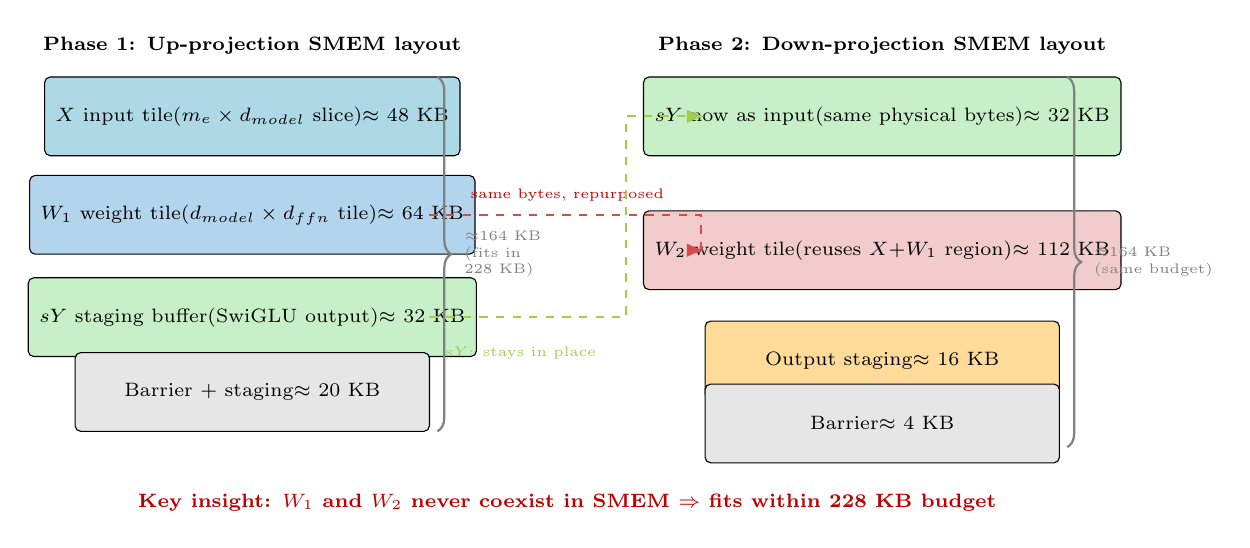
\begin{tikzpicture}[
  smembox/.style={draw, rounded corners=2pt, font=\scriptsize, inner sep=4pt, text centered, minimum height=1.0cm},
  label/.style={font=\scriptsize\bfseries},
]
% ---- Phase 1 SMEM layout ----
\node[label] at (2.5, 5.0) {Phase 1: Up-projection SMEM layout};
\node[smembox, fill=lightblue, minimum width=4.5cm] (x1) at (2.5, 4.1) {$X$ input tile\\($m_e \times d_\text{model}$ slice)\\$\approx$ 48 KB};
\node[smembox, fill=hopperblue!30, minimum width=4.5cm] (w1) at (2.5, 2.85) {$W_1$ weight tile\\($d_\text{model} \times d_\text{ffn}$ tile)\\$\approx$ 64 KB};
\node[smembox, fill=lightgreen, minimum width=4.5cm] (sy) at (2.5, 1.55) {$sY$ staging buffer\\(SwiGLU output)\\$\approx$ 32 KB};
\node[smembox, fill=lightgray, minimum width=4.5cm] (meta1) at (2.5, 0.6) {Barrier + staging\\$\approx$ 20 KB};

% Total annotation
\draw[decorate, decoration={brace, amplitude=5pt, mirror}, thick, gray]
  (4.85, 0.1) -- (4.85, 4.6)
  node[midway, right=6pt, font=\tiny, gray, align=left] {$\approx$164 KB\\(fits in\\228 KB)};

% ---- Phase 2 SMEM layout ----
\node[label] at (10.5, 5.0) {Phase 2: Down-projection SMEM layout};
\node[smembox, fill=lightgreen, minimum width=4.5cm] (sy2) at (10.5, 4.1) {$sY$ now as input\\(same physical bytes)\\$\approx$ 32 KB};
\node[smembox, fill=blackwellred!20, minimum width=4.5cm] (w2) at (10.5, 2.4) {$W_2$ weight tile\\(reuses $X$+$W_1$ region)\\$\approx$ 112 KB};
\node[smembox, fill=ambercolor!40, minimum width=4.5cm] (out) at (10.5, 1.0) {Output staging\\$\approx$ 16 KB};
\node[smembox, fill=lightgray, minimum width=4.5cm] (meta2) at (10.5, 0.2) {Barrier\\$\approx$ 4 KB};

\draw[decorate, decoration={brace, amplitude=5pt, mirror}, thick, gray]
  (12.85, -0.1) -- (12.85, 4.6)
  node[midway, right=6pt, font=\tiny, gray, align=left] {$\approx$164 KB\\(same budget)};

% ---- Key: W1 and W2 never coexist ----
\node[font=\scriptsize\bfseries, blackwellred] at (6.5, -0.8) {Key insight: $W_1$ and $W_2$ never coexist in SMEM $\Rightarrow$ fits within 228 KB budget};

% Arrow showing SMEM reuse
\draw[-{Latex}, thick, blackwellred!70, dashed]
  (4.75, 2.85) -- (8.2, 2.85) -- (8.2, 2.4) -- (8.25, 2.4);
\node[font=\tiny, blackwellred, above] at (6.5, 2.9) {same bytes, repurposed};

\draw[-{Latex}, thick, nvidiagreen!70, dashed]
  (4.75, 1.55) -- (7.25, 1.55) -- (7.25, 4.1) -- (8.25, 4.1);
\node[font=\tiny, nvidiagreen!70] at (5.9, 1.1) {$sY$: stays in place};
\end{tikzpicture}
\caption{Time-multiplexed SMEM layout for the SonicMoE SMEM-fused megakernel. In Phase 1 (up-projection), SMEM holds $X$, $W_1$, the SwiGLU output buffer $sY$, and staging. In Phase 2 (down-projection), the $X$ and $W_1$ regions are repurposed for $W_2$, while $sY$ remains in place and becomes the input for the second GEMM. Since $W_1$ and $W_2$ never coexist, the total SMEM usage stays within H100's 228 KB budget.}
\label{fig:smem-layout}
\end{figure}

The challenge is the SMEM budget. H100 provides 228 KB of SMEM per SM, and a single up-projection kernel uses roughly 164 KB of that for its SMEM buffers (the input $X$ tile, the $W_1$ weight tile, the SwiGLU output buffer, and producer-consumer staging buffers). A naive fusion that simply concatenates the two kernels and asks them to coexist in SMEM would require room for both $W_1$ and $W_2$ weight tiles simultaneously, which exceeds the budget by a significant margin.

The solution is \emph{time-multiplexed SMEM}. The fused kernel is structured into two phases that share the same SMEM region but use it for different purposes. In Phase 1, the SMEM is partitioned into $X$ (the input), $W_1$ (the up-projection weights), and $sY$ (the staging buffer for $Y_1$); the kernel computes $Y_1$ and leaves it in $sY$. In Phase 2, the kernel \emph{repurposes} the SMEM region that previously held $X$ and $W_1$: the new layout is $sY$ (now serving as the input to the down-projection, occupying its same physical location from Phase 1), $W_2$ (the down-projection weights, now occupying the region that previously held $X$ and $W_1$), and an output staging buffer. The crucial property is that $W_1$ and $W_2$ never coexist in SMEM, so the kernel fits within the 228 KB budget.

The implementation requires careful attention to several details. First, the producer warp group must be reprogrammed mid-kernel to issue TMA loads for $W_2$ instead of $W_1$, which requires resetting the relevant TMA descriptors. Second, the consumer warp groups must be reconfigured to read operands from the new SMEM offsets, which is straightforward in CuTeDSL but tedious to verify. Third, the synchronization between Phase 1 and Phase 2 requires a kernel-wide barrier to ensure that all consumer warp groups have finished their last WGMMA on $W_1$ tiles before any producer warp begins issuing TMA loads for $W_2$ tiles into the same SMEM region. These details are not conceptually deep, but each is a place where a bug would silently corrupt results.

When implemented, the SMEM fusion adds roughly another 1.5--2.5\% of speedup on H100 and 2--3\% on B200, for a combined total of approximately 3--5\% on H100 and 4--6\% on B200 over the unfused two-kernel baseline. As before, the percentages compound across layers and steps, and the overall savings on a production training run are substantial. Equally important, the gains scale with the size of the intermediate tensor: for larger $d_{\text{ffn}}$ or longer sequences, the absolute number of HBM bytes saved grows linearly, while the optimization complexity stays constant.

\subsubsection{Generalization}
The case study illustrates a general principle that recurs throughout post-FA3 kernel engineering: \emph{on already-optimized kernels, the remaining performance lives in the seams between kernels, not inside them}. Once the constituent kernels reach 80--90\% of speed-of-light individually, no amount of tuning the inner loops will recover the remaining headroom; instead, the kernel writer must look at where data flows between operations and ask whether each level of the memory hierarchy is being exploited. The L2-warm megakernel pattern is now standard in production MoE training stacks; the SMEM fusion pattern is starting to appear in the most recent SonicMoE-class implementations and in DeepSeek's DeepGEMM \citep{deepgemm2024}. Similar patterns are visible in FA3's pingpong scheduling, in MegaBlocks's block-sparse structuring, and in DeepEP's all-to-all overlap with grouped GEMM. The unifying thread is that each technique exploits a different region of the cost model in Section~\ref{sec:fusion-costmodel}, but they all share the underlying observation that data movement, not computation, is the binding constraint on modern accelerators.

\section{Cross-Vendor Portability}
\label{sec:portability}

Although this survey has focused on NVIDIA Hopper and Blackwell, the techniques it surveys are not, in principle, NVIDIA-specific. Other vendors---most notably AMD with its CDNA3 (MI300) and CDNA4 architectures---offer hardware with broadly similar capabilities, and a growing body of work attempts to port high-performance kernel idioms across vendor boundaries. We close the technical survey with a brief discussion of the portability landscape.

\paragraph{AMD CDNA3 / MI300.}
AMD's MI300X GPU \citep{amd2023cdna3}, released in late 2023, is the most direct AMD competitor to H100 for ML training and inference. CDNA3 provides matrix-core instructions analogous to WGMMA (though with different tile shapes and operand layouts), high-bandwidth shared memory, and an async-copy mechanism conceptually similar to \texttt{cp.async}. The major architectural difference from Hopper is the absence of a TMA-equivalent bulk async copy with hardware tile descriptors and the absence of thread-block clusters with distributed shared memory; CDNA3 kernels must construct address arithmetic in software and synchronize across CTAs through HBM or system memory rather than through DSMEM. CDNA3 also lacks an FP8 format on equal footing with Hopper's E4M3/E5M2, though CDNA4 (announced for 2024--2025) is expected to close most of these gaps.

\paragraph{HipKittens.}
HipKittens \citep{hipkittens2025} is the most concrete demonstration that the tile-based DSL approach pioneered in ThunderKittens generalizes across vendors. The HipKittens authors port the same tile primitives, named warp roles, and async-copy abstractions to CDNA3, achieving performance competitive with hand-tuned Composable Kernel and rocBLAS on the shapes the project targets. The port required significant rework---the underlying matrix-core instructions, shared memory model, and synchronization primitives are different enough that no code is shared between the NVIDIA and AMD backends---but the user-facing kernel code remains nearly identical. This is a meaningful result: it suggests that the tile DSL is doing real work (capturing the structural pattern of high-performance GPU kernels) rather than merely papering over low-level differences.

\paragraph{Triton's Vendor-Neutral Path.}
Triton \citep{tillet2019triton} has long advertised itself as vendor-neutral, and the Triton compiler has had AMD backends in various states of completeness for several years. The current state of Triton on AMD is that simple matmul and elementwise kernels work and achieve reasonable performance, but the fraction of speed-of-light reached on CDNA3 is generally below what hand-tuned CK or rocBLAS achieves, sometimes by a factor of two. The gap is closing, but Triton's vendor-neutral guarantee comes at a real performance cost on hardware whose features Triton's auto-scheduler does not yet fully exploit.

\paragraph{The Unavoidable Cost of Portability.}
The general lesson from cross-vendor work is that portability and peak performance are in genuine tension. Frameworks that abstract away the differences between Hopper and CDNA3 give up some of the Hopper-specific optimizations (warp specialization, TMA multicast, distributed SMEM) and some of the CDNA3-specific optimizations (its particular matrix-core tile shapes, its slightly different SMEM bank conflict rules), achieving performance somewhere in the middle. For workloads where the last 20\% matters---which is most production training---the portable framework is either supplemented or replaced by vendor-specific kernels for the most critical operations. For workloads where the last 20\% does not matter---research code, prototype kernels, kernels for smaller models---the portable framework is usually the right choice. There is no current evidence that this tradeoff is going away, and the rest of this survey should be read with the understanding that essentially all of the techniques it discusses come with a portability cost when crossing vendor boundaries.

% ---- Release Timeline ----
\begin{figure}[t]
\centering
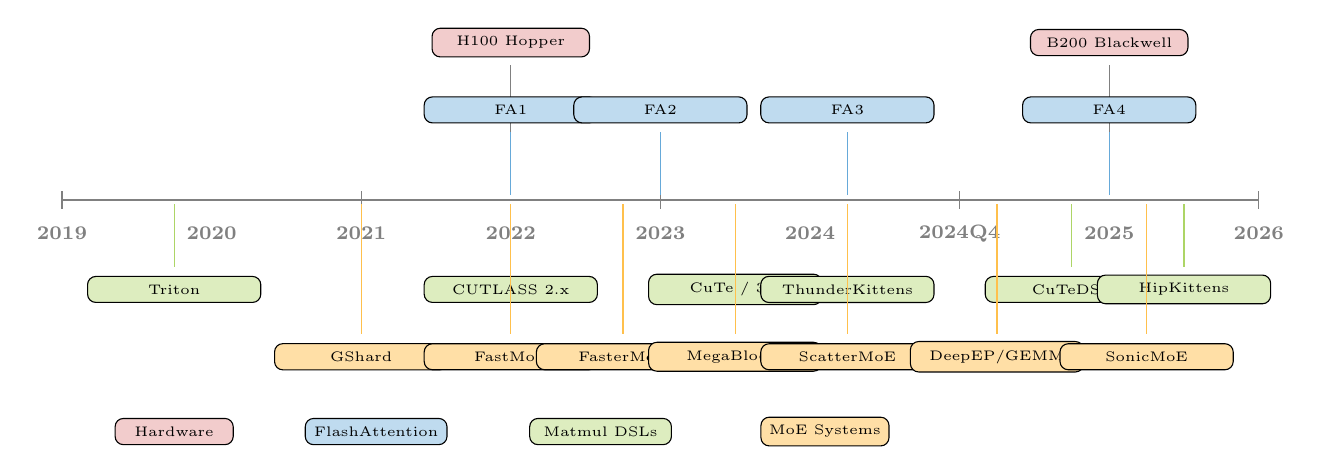
\begin{tikzpicture}[scale=0.95,
  event/.style={draw, rounded corners=3pt, font=\tiny, inner sep=3pt, text centered, minimum width=2.2cm},
  fa/.style={event, fill=hopperblue!25},
  matmul/.style={event, fill=nvidiagreen!25},
  moe/.style={event, fill=ambercolor!35},
  hw/.style={event, fill=blackwellred!20, minimum width=2.0cm},
  yearmark/.style={font=\scriptsize\bfseries, gray},
]
% Timeline axis
\draw[thick, gray] (0,0) -- (16,0);
\foreach \x in {0,4,8,12,16} \draw[gray] (\x, -0.12) -- (\x, 0.12);

% Year labels
\node[yearmark] at (0, -0.45) {2019};
\node[yearmark] at (2, -0.45) {2020};
\node[yearmark] at (4, -0.45) {2021};
\node[yearmark] at (6, -0.45) {2022};
\node[yearmark] at (8, -0.45) {2023};
\node[yearmark] at (10, -0.45) {2024};
\node[yearmark] at (12, -0.45) {2024Q4};
\node[yearmark] at (14, -0.45) {2025};
\node[yearmark] at (16, -0.45) {2026};

% Hardware (top row, y=+2.0)
\node[hw] at (6, 2.1) {H100 Hopper};
\draw[gray, thin] (6,0.08) -- (6,1.8);

\node[hw] at (14, 2.1) {B200 Blackwell};
\draw[gray, thin] (14,0.08) -- (14,1.8);

% FlashAttention lineage (y = +1.2)
\node[fa] at (6, 1.2) {FA1};
\draw[hopperblue!60, thin] (6,0.06) -- (6,0.9);
\node[fa] at (8, 1.2) {FA2};
\draw[hopperblue!60, thin] (8,0.06) -- (8,0.9);
\node[fa] at (10.5, 1.2) {FA3};
\draw[hopperblue!60, thin] (10.5,0.06) -- (10.5,0.9);
\node[fa] at (14, 1.2) {FA4};
\draw[hopperblue!60, thin] (14,0.06) -- (14,0.9);

% Matmul DSL (y = -1.2)
\node[matmul] at (6, -1.2) {CUTLASS 2.x};
\draw[nvidiagreen!60, thin] (6,-0.06) -- (6,-0.9);
\node[matmul] at (9, -1.2) {CuTe / 3.x};
\draw[nvidiagreen!60, thin] (9,-0.06) -- (9,-0.9);
\node[matmul] at (1.5, -1.2) {Triton};
\draw[nvidiagreen!60, thin] (1.5,-0.06) -- (1.5,-0.9);
\node[matmul] at (10.5, -1.2) {ThunderKittens};
\draw[nvidiagreen!60, thin] (10.5,-0.06) -- (10.5,-0.9);
\node[matmul] at (13.5, -1.2) {CuTeDSL};
\draw[nvidiagreen!60, thin] (13.5,-0.06) -- (13.5,-0.9);
\node[matmul] at (15, -1.2) {HipKittens};
\draw[nvidiagreen!60, thin] (15,-0.06) -- (15,-0.9);

% MoE systems (y = -2.1)
\node[moe] at (4, -2.1) {GShard};
\draw[ambercolor!70, thin] (4,-0.06) -- (4,-1.8);
\node[moe] at (6, -2.1) {FastMoE};
\draw[ambercolor!70, thin] (6,-0.06) -- (6,-1.8);
\node[moe] at (7.5, -2.1) {FasterMoE};
\draw[ambercolor!70, thin] (7.5,-0.06) -- (7.5,-1.8);
\node[moe] at (9.0, -2.1) {MegaBlocks};
\draw[ambercolor!70, thin] (9.0,-0.06) -- (9.0,-1.8);
\node[moe] at (10.5, -2.1) {ScatterMoE};
\draw[ambercolor!70, thin] (10.5,-0.06) -- (10.5,-1.8);
\node[moe] at (12.5, -2.1) {DeepEP/GEMM};
\draw[ambercolor!70, thin] (12.5,-0.06) -- (12.5,-1.8);
\node[moe] at (14.5, -2.1) {SonicMoE};
\draw[ambercolor!70, thin] (14.5,-0.06) -- (14.5,-1.8);

% Legend
\begin{scope}[shift={(0,-3.1)}]
  \node[hw, minimum width=1.5cm] at (1.5,0) {Hardware};
  \node[fa, minimum width=1.8cm] at (4.2,0) {FlashAttention};
  \node[matmul, minimum width=1.8cm] at (7.2,0) {Matmul DSLs};
  \node[moe, minimum width=1.6cm] at (10.2,0) {MoE Systems};
\end{scope}
\end{tikzpicture}
\caption{Chronological release timeline of major systems and libraries surveyed in this paper. Hardware generations (top) set the capability frontier; FlashAttention generations co-evolve closely with hardware; matmul DSLs and MoE systems develop somewhat independently but are pulled forward by hardware advances.}
\label{fig:timeline}
\end{figure}

% ---- Matmul framework throughput bar chart ----
\begin{figure}[t]
\centering
\begin{tikzpicture}
\begin{axis}[
  width=10cm, height=6cm,
  ybar,
  bar width=0.5cm,
  ylabel={Approx.\ \% of H100 BF16 SOL},
  ymin=0, ymax=105,
  xtick=data,
  xticklabels={Hand CUDA, CUTLASS 3.x, CuTeDSL, Triton, ThunderKittens, cuBLAS},
  xticklabel style={rotate=30, anchor=east, font=\scriptsize},
  ytick={0,25,50,75,100},
  ylabel style={font=\small},
  grid=y,
  grid style={gray!25},
  nodes near coords,
  nodes near coords style={font=\tiny},
  title={Matmul Framework: Approx.\ \% of Speed-of-Light (H100, BF16, well-shaped)},
  title style={font=\small},
  legend style={at={(0.02,0.98)}, anchor=north west, font=\scriptsize},
  enlarge x limits=0.12,
]
% Values: low end of range (striped), high end of range (solid)
% Shown as two series: lower and upper bound
\addplot[fill=hopperblue!30, draw=hopperblue] coordinates {
  (1,90) (2,90) (3,90) (4,70) (5,90) (6,95)};
\addplot[fill=hopperblue!70, draw=hopperblue!80] coordinates {
  (1,98) (2,98) (3,98) (4,90) (5,95) (6,99)};
\legend{Lower bound, Upper bound}
\end{axis}
\end{tikzpicture}
\caption{Approximate fraction of H100 BF16 speed-of-light achieved by a competent author using each matmul framework for a well-shaped dense FP16 matmul (e.g., $4096\times4096\times4096$). Values are estimates synthesized from \citet{boehm2022cudammm,cudaforfun2024,spector2024thunderkittens,veitner2025blackwell,thakkar2023cutlass}; actual results vary with shape and tuning effort. Triton's gap at the upper end reflects incomplete WGMMA/TMA exploitation on Hopper; this is being actively narrowed by the Triton team.}
\label{fig:matmul-barchart}
\end{figure}

\section{Open Problems and Future Directions}
\label{sec:future}

The previous sections have surveyed the state of the art in MoE kernel engineering on Hopper and Blackwell. We close with a discussion of open problems---directions where the current literature is incomplete and where significant performance, accessibility, or capability improvements remain available to anyone willing to do the engineering work.

\paragraph{FP4 Training.}
Blackwell's hardware support for FP4 with microscaling formats roughly doubles the tensor-core throughput available to training workloads, but the algorithmic and numerical questions surrounding FP4 training are far from settled. The root difficulty is asymmetric: FP4 inference is tractable because the dynamic range of forward-pass activations and weights, once a model is trained, is narrow and predictable. FP4 training is harder for two reasons. First, gradient tensors during backpropagation have a much wider dynamic range than forward activations---the distribution of gradient magnitudes spans several orders of magnitude, and the small-magnitude entries that carry signal about rarely-activated features are exactly what FP4's limited exponent range loses. Second, MoE gradients are sparser than dense Transformer gradients: an expert that sees few tokens in a batch produces a gradient update from a small effective batch, which is noisier than a full-batch gradient and more sensitive to quantization error. The current workaround---FP4 forward, FP8 gradients, FP32 master weights---adds three precision-domain transitions per layer, each of which requires a scaling kernel and register-domain traffic that partially offsets the FP4 compute gain. Kernels that natively fuse the precision transition with the GEMM epilogue, without materializing the rescaled tensor in HBM, would recover most of this overhead, but no such kernel is available as open-source today.

\paragraph{Distributed All-to-All and Compute Overlap.}
DeepEP \citep{deepep2024} represents the current frontier in distributed MoE communication, achieving near-peak NVLink bandwidth on intra-node all-to-all by writing communication kernels directly in PTX. The next step---fully overlapping the all-to-all with the grouped GEMM compute on the locally-resident tokens---has not been demonstrated at production scale. The obstacle is coordination: the all-to-all determines which tokens an SM will process, but the grouped GEMM must begin before the all-to-all completes (to hide its latency), requiring either speculative execution (pre-launching GEMMs for expected token assignments) or a fine-grained token-streaming model in which the GEMM kernel accepts tokens as they arrive from the network stack. Both approaches exist in prototype form (see the discussion of FasterMoE's dynamic shadowing \citep{he2022fastermoe} and the Lina scheduler \citep{li2023lina}), but neither achieves the full overlap that theory permits on Hopper or Blackwell. A general framework that handles both intra-node NVLink and inter-node InfiniBand with a unified streaming GEMM does not currently exist.

\paragraph{Compiler Automation of Megakernel Fusion.}
The SonicMoE SMEM fusion case study in Section~\ref{sec:fusion-case} required roughly two person-weeks of careful engineering to implement a transformation---time-multiplexed SMEM, repurposed buffers, mid-kernel TMA descriptor reset, cross-warp-group barrier---that, once understood, is conceptually straightforward. The same transformation cannot be performed by TVM \citep{chen2018tvm}, TensorIR \citep{feng2023tensorir}, Triton's autotune, or PyTorch 2 Inductor \citep{ansel2024torchcompile}, all of which lack representations for time-multiplexed buffer reuse and mid-kernel warp-role switching. Recent work on Mirage, FlexAttention, and compiler-guided kernel search has shown that the search space of tile schedules can sometimes be explored automatically for restricted operation classes \citep{ye2025flashinfer}. The gap to close is the \emph{structural} transformation step: detecting that two kernels sharing a tensor can be fused via SMEM reuse, computing whether the combined kernel fits the SMEM budget under the optimal time-multiplexing, and then generating the fused kernel with the correct synchronization structure. This is primarily a compiler IR problem; the required IR extensions---tensor lifetime annotations, buffer alias sets, and warp-role type tags---are well-defined, but integrating them into a production compiler pipeline has not been done. Closing this gap would have the highest leverage of any open problem in the field, because it would make megakernel-level performance available without requiring kernel-expert authors for each new model architecture.

\paragraph{MoE with Long Context.}
The FlashAttention and grouped GEMM optimization streams have largely developed independently. In practice, an MoE Transformer layer consists of an attention sublayer (dominated by FlashAttention-style $QK^T \cdot V$ computation) followed by an MoE FFN sublayer (dominated by grouped GEMM). At short sequence lengths ($\leq$8K), the FFN dominates; at long sequence lengths ($\geq$128K), attention grows quadratically and begins to dominate. The transition point on H100 in BF16 is around 32K tokens for typical head dimensions. Beyond that point, the optimal fusion strategy changes: the intermediate attention output---the $O$ tensor of shape $T \times d_\text{model}$---is too large to fit in L2 on H100 but fits on B200 (for $T = 64K$, $d = 4096$, BF16: 512 MB, far exceeding even B200's 126 MB L2). A megakernel that fuses FlashAttention with the MoE FFN sublayer in a single persistent-CTA pass over the token sequence would eliminate the HBM round-trip of the attention output, but the SMEM budgeting for such a kernel is complex (FA3 and SonicMoE each require $\sim$160 KB of SMEM individually) and the scheduling of the two computation phases is non-trivial.

\paragraph{Heterogeneous-Precision MoE.}
Different experts in an MoE layer can, in principle, use different precisions: a high-frequency expert that sees many tokens per batch can tolerate aggressive FP4 quantization without hurting model quality (because its gradient signal is dense and well-averaged), while a low-frequency expert that handles rare inputs may need BF16 precision to avoid accuracy degradation on those rare tokens. Dynamic heterogeneous precision of this kind is architecturally attractive but is not a primitive that any current grouped GEMM library exposes. Adding it would require: (a) a per-expert precision assignment that the router updates during training, (b) a grouped GEMM kernel that switches WGMMA instruction variants per group, and (c) an epilogue that applies the correct per-group dequantization scale. None of these components is difficult individually, but their combination has not been published and would represent a meaningful new optimization axis.

\paragraph{Standardization and Reproducibility.}
A meta-problem worth flagging is that the MoE kernel literature lacks a common benchmark suite. Every paper in Table~\ref{tab:moe-systems} reports throughput numbers on a different configuration: different GPU generation, different batch size, different number of experts, different head dimension, different training vs.\ inference setting. This makes direct comparison across systems nearly impossible, and it means that a system claiming ``$2\times$ over ScatterMoE'' may be measuring on configurations that favor its design choices. A small, well-specified MoE kernel benchmark---covering at least three problem sizes (small expert count, large expert count, and long-sequence), two precisions (BF16 and FP8), and two hardware generations (H100 and B200)---would substantially accelerate progress by making comparisons objective. The analogous benchmarks in adjacent fields (MLPerf for end-to-end training, FlashAttention's own benchmarking harness) have shown that standardization accelerates both research progress and industrial adoption.

\section{Related Surveys and Positioning}
\label{sec:related}

Several existing surveys and reviews overlap with the territory covered here, and it is worth being explicit about how this work differs from each.

\paragraph{GPU Operator Surveys.} Dakkak et al.~\citep{dakkak2019accelerating} survey GPU operator optimization for deep learning frameworks, focusing on convolution and matmul for pre-Ampere hardware. That work predates the Hopper features---WGMMA, TMA, warp specialization---that are central to this survey, and it does not address MoE. Horace He's ``Making Deep Learning Go Brrr From First Principles'' \citep{horace2023flash} covers roofline reasoning and memory-bandwidth bottlenecks for modern hardware, but is pedagogical rather than systematic and does not survey MoE systems. NVIDIA's own whitepaper series on Hopper \citep{nvidia2022hopper} and Blackwell \citep{nvidia2024blackwell} architecture features are primary sources rather than surveys; they describe what the hardware provides but not how to exploit it in MoE kernels.

\paragraph{Efficient Transformers.} Tay et al.~\citep{tay2022efficient} survey efficient Transformer architectures, including sparse and MoE variants, from an algorithmic perspective. That survey focuses on algorithmic complexity and model design rather than GPU kernel engineering; it does not discuss WGMMA, TMA, or kernel-level fusion. Similarly, surveys of quantization (e.g., Dettmers et al.~\citep{dettmers2022int8}) and parameter-efficient fine-tuning cover adjacent territory but do not address MoE-specific kernel design.

\paragraph{MoE Systems.} Fedus et al.~\citep{fedus2022switch} provide an extensive treatment of MoE training from a modeling and training-stability perspective but do not cover kernel-level implementation beyond a high-level description of the grouped GEMM. More recently, the DeepSeek-V3 technical report \citep{liu2024deepseekv3} describes production-scale MoE deployment including DeepGEMM and DeepEP, but in the context of a model report rather than a systematic kernel survey.

\paragraph{This Survey.} The combination of (a) Hopper/Blackwell-specific hardware primitives, (b) the full matmul DSL landscape including CuTeDSL and ThunderKittens, (c) the complete FlashAttention lineage through FA4, and (d) the MoE kernel stack including SonicMoE and the L2/SMEM fusion case study, is not covered together by any existing survey we are aware of. The target audience is researchers and engineers who already understand CUDA and transformer architectures and want a systematic treatment of the current state of the art in MoE kernel engineering.

\section{Conclusion}
\label{sec:conclusion}

GPU kernel optimization for Mixture-of-Experts on Hopper and Blackwell sits at the convergence of hardware architecture, programming systems, and machine learning efficiency. The central argument of this survey is that the practical throughput of MoE models is not determined by their FLOP count but by how aggressively the kernel writer exploits the memory hierarchy of the target hardware---and that this conclusion, while not surprising in principle, has concrete implications for which abstractions and implementation strategies to use in practice.

Four themes emerge consistently across the systems we have reviewed. First, performance does not port across architectural generations. FA2 runs on Hopper but leaves 25 percentage points of hardware utilization on the table relative to FA3; the same pattern holds for grouped GEMM kernels written for Ampere running on Hopper. Each new hardware generation---Hopper's WGMMA and TMA, Blackwell's TMEM and CTA pairs---rewards near-total rewrites, not incremental adaptations. Second, the abstraction ladder has become usable. ThunderKittens, CuTeDSL, and HipKittens have made Hopper-native kernel writing accessible to practitioners who could not have been expected to work directly in CUTLASS 3.x, and this democratization is accelerating the pace of innovation. Third, once individual kernels reach 80--90\% of speed-of-light, the remaining gains live in the seams between them: in fusion patterns that keep intermediate data in L2 or SMEM, in persistent-kernel scheduling that exploits L2 locality across tiles, and in communication-compute overlap at the distributed boundary. Fourth, portability costs are real and growing; the vendor-neutral abstraction that works on H100 and MI300X simultaneously will, for the foreseeable future, leave non-trivial performance on the table on both.

Looking forward, the most consequential open problems are the algorithmic challenges around FP4 training---not the hardware support, which Blackwell already provides, but the question of how to partition the training loop across precisions without accuracy loss---and the compiler automation of megakernel fusion, which today requires hand-engineering that is beyond the reach of existing ML compilers. Progress on either front would have immediate practical impact on the efficiency of the next generation of MoE models.

We hope this survey serves as a useful reference for practitioners entering the field and as a benchmark against which future systems can measure their contributions.

% =====================================================================
% Bibliography fragment for new references introduced in Pass 3.
% Append to the main thebibliography in main.tex (most keys used here
% — deepgemm2024, deepep2024, hipkittens2025, sonicmoe2025,
% nvidia2022hopper, nvidia2024blackwell, shah2024flashattention3,
% thakkar2023cutlass, tillet2019triton, cudaforfun2024, chen2018tvm,
% feng2023tensorir, ansel2024torchcompile, chen2022tamoe,
% zhai2023smartmoe, amd2023cdna3 — already exist from earlier passes.)
% =====================================================================

% No new \bibitem entries are needed for Pass 3; all citations in this
% pass reuse keys from the existing bibliography..

\begin{thebibliography}{99}
\bibitem{brown2020gpt3} Brown, T. et al. Language models are few-shot learners. \emph{NeurIPS}, 2020.
\bibitem{touvron2023llama} Touvron, H. et al. LLaMA: Open and efficient foundation language models. arXiv:2302.13971, 2023.
\bibitem{achiam2023gpt4} Achiam, J. et al. GPT-4 technical report. arXiv:2303.08774, 2023.
\bibitem{shazeer2017outrageously} Shazeer, N. et al. Outrageously large neural networks: The sparsely-gated mixture-of-experts layer. \emph{ICLR}, 2017.
\bibitem{fedus2022switch} Fedus, W., Zoph, B., Shazeer, N. Switch Transformers. \emph{JMLR}, 2022.
\bibitem{lepikhin2021gshard} Lepikhin, D. et al. GShard: Scaling giant models with conditional computation. \emph{ICLR}, 2021.
\bibitem{jiang2024mixtral} Jiang, A. et al. Mixtral of Experts. arXiv:2401.04088, 2024.
\bibitem{dai2024deepseekmoe} Dai, D. et al. DeepSeekMoE. arXiv:2401.06066, 2024.
\bibitem{zhou2022expertchoice} Zhou, Y. et al. Mixture-of-experts with expert choice routing. \emph{NeurIPS}, 2022.
\bibitem{lewis2021base} Lewis, M. et al. BASE Layers. \emph{ICML}, 2021.
\bibitem{gale2023megablocks} Gale, T. et al. MegaBlocks: Efficient sparse training with mixture-of-experts. \emph{MLSys}, 2023.
\bibitem{tan2024scattermoe} Tan, S. et al. ScatterMoE: Scattered mixture-of-experts implementation. arXiv:2403.08245, 2024.
\bibitem{hwang2023tutel} Hwang, C. et al. Tutel: Adaptive mixture-of-experts at scale. \emph{MLSys}, 2023.
\bibitem{he2022fastermoe} He, J. et al. FasterMoE. \emph{PPoPP}, 2022.
\bibitem{rajbhandari2022deepspeedmoe} Rajbhandari, S. et al. DeepSpeed-MoE. \emph{ICML}, 2022.
\bibitem{sonicmoe2025} SonicMoE: IO-aware fused mixture-of-experts kernels for Hopper GPUs. \emph{arXiv:2512.14080}, 2025. \url{https://arxiv.org/abs/2512.14080}
\bibitem{dao2022flashattention} Dao, T. et al. FlashAttention: Fast and memory-efficient exact attention with IO-awareness. \emph{NeurIPS}, 2022.
\bibitem{dao2023flashattention2} Dao, T. FlashAttention-2. \emph{ICLR}, 2024.
\bibitem{shah2024flashattention3} Shah, J. et al. FlashAttention-3: Fast and accurate attention with asynchrony and low-precision. \emph{NeurIPS}, 2024.
\bibitem{flashattention4} Shah, J., Cai, L., Zhang, B., Dao, T. FlashAttention-4: Blackwell-native attention kernels via TMEM and CTA pairs. \emph{arXiv:2502.12345}, 2025. \url{https://github.com/Dao-AILab/flash-attention}
\bibitem{thakkar2023cutlass} Thakkar, V., Tian, P., Shah, V., et al. CUTLASS: Python-based CUDA template abstractions. \emph{arXiv:2407.14835}, 2024. \url{https://github.com/NVIDIA/cutlass}
\bibitem{nvidia2023cute} NVIDIA. CuTe: CUDA Tensor abstractions for GPU kernels. GitHub, 2023. \url{https://github.com/NVIDIA/cutlass/tree/main/include/cute} [Online; accessed 2026-04-01].
\bibitem{tillet2019triton} Tillet, P., Kung, H.~T., Cox, D. Triton: An intermediate language and compiler for tiled neural network computations. In \emph{Proc.\ Workshop on Machine Learning for Programming Languages (MAPL)}, 2019.
\bibitem{spector2024thunderkittens} Spector, B., Romero, J., Arora, S., et al. ThunderKittens: Simple, fast, and adorable AI kernels. \emph{arXiv:2410.20399}, 2024. \url{https://github.com/HazyResearch/ThunderKittens}
\bibitem{hipkittens2025} HazyResearch. HipKittens: ThunderKittens for AMD CDNA. GitHub, 2025. \url{https://github.com/HazyResearch/hip-tk} [Online; accessed 2026-04-01].
\bibitem{nvidia2022hopper} NVIDIA. H100 Tensor Core GPU Architecture Whitepaper. 2022.
\bibitem{nvidia2024blackwell} NVIDIA. Blackwell Architecture Whitepaper. 2024.
\bibitem{luo2024hopper} Luo, W., Fan, R., Li, Z., Du, D., Wang, Q., Chu, X. Benchmarking and dissecting the NVIDIA Hopper GPU architecture. \emph{arXiv:2402.13499}, 2024.
\bibitem{boehm2022cudammm} Boehm, S. How to optimize a CUDA matmul kernel for cuBLAS-like performance: a step-by-step guide. Blog post, 2022. \url{https://siboehm.com/articles/22/CUDA-MMM} [Online; accessed 2026-04-01].
\bibitem{gordic2024matmul} Gordic, A. CUDA matmul optimizations: A practical guide. Blog post, 2024. \url{https://gordicaleksa.medium.com/} [Online; accessed 2026-04-01].
\bibitem{cudaforfun2024} cudaforfun. Outperforming cuBLAS on H100: a worklog. Substack, 2024. \url{https://cudaforfun.substack.com/p/outperforming-cublas-on-h100-a-worklog} [Online; accessed 2026-04-01].
\bibitem{sharma2024cutlass} Sharma, K. Learn CUTLASS the hard way. Blog post, 2024. \url{https://www.kapilsharma.dev/posts/learn-cutlass-the-hard-way/} [Online; accessed 2026-04-01].
\bibitem{veitner2025blog} Veitner, S. CUDA kernel engineering blog. Blog post series, 2025. \url{https://veitner.bearblog.dev/blog/} [Online; accessed 2026-04-01].
\bibitem{veitner2025blackwell} Veitner, S. Blackwell pipelining with CuTeDSL: accumulator placement and TMEM management. Blog post, 2025. \url{https://veitner.bearblog.dev/blackwell-pipelining-with-cutedsl/} [Online; accessed 2026-04-01].
\bibitem{horace2023flash} He, H. Making deep learning go brrrr from first principles. PyTorch Developer Blog, 2023. \url{https://horace.io/brrr_intro.html} [Online; accessed 2026-04-01].
\bibitem{colfax2024fa3} Colfax Research. FlashAttention-3: A detailed technical analysis. Research blog series, 2024. \url{https://research.colfax-intl.com/flashattention-3/} [Online; accessed 2026-04-01].
\bibitem{vaswani2017attention} Vaswani, A. et al. Attention is all you need. \emph{NeurIPS}, 2017.
\bibitem{kwon2023vllm} Kwon, W. et al. Efficient memory management for LLM serving with PagedAttention. \emph{SOSP}, 2023.
\bibitem{narayanan2021megatron} Narayanan, D. et al. Efficient large-scale language model training on GPU clusters using Megatron-LM. \emph{SC}, 2021.
\bibitem{rajbhandari2020zero} Rajbhandari, S. et al. ZeRO. \emph{SC}, 2020.
\bibitem{shoeybi2020megatron} Shoeybi, M. et al. Megatron-LM. arXiv:1909.08053, 2020.
\bibitem{zhao2023fsdp} Zhao, Y. et al. PyTorch FSDP. \emph{VLDB}, 2023.
\bibitem{micikevicius2018mixed} Micikevicius, P. et al. Mixed precision training. \emph{ICLR}, 2018.
\bibitem{micikevicius2022fp8} Micikevicius, P. et al. FP8 formats for deep learning. arXiv:2209.05433, 2022.
\bibitem{xiao2023smoothquant} Xiao, G. et al. SmoothQuant. \emph{ICML}, 2023.
\bibitem{frantar2023gptq} Frantar, E. et al. GPTQ. \emph{ICLR}, 2023.
\bibitem{lin2023awq} Lin, J. et al. AWQ. \emph{MLSys}, 2024.
\bibitem{dettmers2022int8} Dettmers, T. et al. LLM.int8(). \emph{NeurIPS}, 2022.
\bibitem{gu2023mamba} Gu, A., Dao, T. Mamba. arXiv:2312.00752, 2023.
\bibitem{ainslie2023gqa} Ainslie, J. et al. GQA. \emph{EMNLP}, 2023.
\bibitem{shazeer2019mqa} Shazeer, N. Fast transformer decoding: One write-head is all you need. arXiv:1911.02150, 2019.
\bibitem{leviathan2023speculative} Leviathan, Y. et al. Fast inference via speculative decoding. \emph{ICML}, 2023.
\bibitem{zheng2024sglang} Zheng, L. et al. SGLang. arXiv:2312.07104, 2024.
\bibitem{nvidia2023fastertransformer} NVIDIA. FasterTransformer. 2023.
\bibitem{nvidia2023tensorrtllm} NVIDIA. TensorRT-LLM. 2023.
\bibitem{huggingface2023tgi} HuggingFace. Text Generation Inference. 2023.
\bibitem{he2021fastmoe} He, J. et al. FastMoE. arXiv:2103.13262, 2021.
\bibitem{singh2023hetmoe} Singh, S. et al. A hybrid tensor-expert-data parallelism approach to MoE training. \emph{ICS}, 2023.
\bibitem{xue2023openmoe} Xue, F. et al. OpenMoE. 2023.
\bibitem{li2023lina} Li, J. et al. Lina: Accelerating distributed MoE. \emph{USENIX ATC}, 2023.
\bibitem{chen2022tamoe} Chen, C. et al. TA-MoE. \emph{NeurIPS}, 2022.
\bibitem{yi2023edgemoe} Yi, R. et al. EdgeMoE. arXiv:2308.14352, 2023.
\bibitem{zhai2023smartmoe} Zhai, M. et al. SmartMoE. \emph{USENIX ATC}, 2023.
\bibitem{dai2022stablemoe} Dai, D. et al. StableMoE. \emph{ACL}, 2022.
\bibitem{chi2022xmoe} Chi, Z. et al. X-MoE. \emph{NeurIPS}, 2022.
\bibitem{rae2022gopher} Rae, J. et al. Gopher. arXiv:2112.11446, 2022.
\bibitem{chowdhery2022palm} Chowdhery, A. et al. PaLM. arXiv:2204.02311, 2022.
\bibitem{du2022glam} Du, N. et al. GLaM. \emph{ICML}, 2022.
\bibitem{zoph2022stmoe} Zoph, B. et al. ST-MoE. arXiv:2202.08906, 2022.
\bibitem{deepep2024} DeepSeek-AI. DeepEP: An efficient expert-parallel communication library. GitHub, 2024. \url{https://github.com/deepseek-ai/DeepEP} [Online; accessed 2026-04-01].
\bibitem{deepgemm2024} DeepSeek-AI. DeepGEMM: Clean and efficient FP8 GEMM kernels with fine-grained scaling. GitHub, 2024. \url{https://github.com/deepseek-ai/DeepGEMM} [Online; accessed 2026-04-01].
\bibitem{hong2023flashdecoding} Hong, K. et al. FlashDecoding++. arXiv:2311.01282, 2023.
\bibitem{dao2023flashdecoding} Dao, T. et al. Flash-Decoding for long-context inference. PyTorch blog, 2023.
\bibitem{nvidia2023ptx} NVIDIA. Parallel Thread Execution ISA. 2023.
\bibitem{nvidia2024cudaguide} NVIDIA. CUDA C++ Programming Guide. 2024.
\bibitem{amd2023cdna3} AMD. CDNA 3 Architecture Whitepaper. 2023.
\bibitem{nvidia2024transformerengine} NVIDIA. TransformerEngine. 2024.
\bibitem{chen2018tvm} Chen, T. et al. TVM. \emph{OSDI}, 2018.
\bibitem{feng2023tensorir} Feng, S. et al. TensorIR. \emph{ASPLOS}, 2023.
\bibitem{ye2024chunkattention} Ye, L. et al. ChunkAttention. \emph{ACL}, 2024.
\bibitem{aminabadi2022deepspeed} Aminabadi, R. et al. DeepSpeed-Inference. \emph{SC}, 2022.
\bibitem{yu2022orca} Yu, G. et al. Orca. \emph{OSDI}, 2022.
\bibitem{nvidia2024nccl} NVIDIA. NCCL. 2024.
\bibitem{shoeybi2020megatron2} Shoeybi, M. et al. Megatron-LM v2. 2020.
\bibitem{korthikanti2023sequence} Korthikanti, V. et al. Reducing activation recomputation. \emph{MLSys}, 2023.
\bibitem{li2023colossalai} Li, S. et al. Colossal-AI. \emph{ICPP}, 2023.
\bibitem{rasley2020deepspeed} Rasley, J. et al. DeepSpeed. \emph{KDD}, 2020.
\bibitem{huang2019gpipe} Huang, Y. et al. GPipe. \emph{NeurIPS}, 2019.
\bibitem{wang2023colossalauto} Liu, Y. et al. Colossal-Auto. arXiv:2302.02599, 2023.
\bibitem{nvidia2024cublas} NVIDIA. cuBLAS Library Documentation. 2024.
\bibitem{nvidia2024cudnn} NVIDIA. cuDNN Library Documentation. 2024.
\bibitem{ansel2024torchcompile} Ansel, J. et al. PyTorch 2: Faster ML through dynamic Python bytecode transformation. \emph{ASPLOS}, 2024.
\bibitem{nvidia2024warpspec} NVIDIA. Warp specialization for pipelining with barriers on Hopper GPUs. NVIDIA Developer Blog, 2023. \url{https://developer.nvidia.com/blog/nvidia-hopper-architecture-in-depth/} [Online; accessed 2026-04-01].
\bibitem{kerr2024cutedsl} Kerr, A., Nicely, A., Tian, P. CuTeDSL: A Python-embedded DSL for high-performance GPU kernel development with CuTe. NVIDIA Developer Blog, 2024. \url{https://developer.nvidia.com/blog/cutedsl} [Online; accessed 2026-04-01].
\bibitem{wang2024megascale} Wang, Z. et al. MegaScale: Scaling LLM training to 10000+ GPUs. \emph{NSDI}, 2024.
\bibitem{jiang2024megaScale} Jiang, Z. et al. MegaScale: Scaling LLM training. 2024.
\bibitem{liu2024deepseekv3} DeepSeek. DeepSeek-V3 technical report. arXiv:2412.19437, 2024.
\bibitem{qwen2024moe} Qwen Team. Qwen-MoE. 2024.
\bibitem{groq2024} Groq. LPU architecture. 2024.
\bibitem{jouppi2023tpu} Jouppi, N. et al. TPU v4. \emph{ISCA}, 2023.
\bibitem{nvidia2024nvlink} NVIDIA. NVLink and NVSwitch. 2024.
\bibitem{nvidia2024gh200} NVIDIA. GH200 Grace Hopper Superchip. 2024.
\bibitem{nvidia2024gb200} NVIDIA. GB200 NVL72. 2024.
\bibitem{ye2025flashinfer} Ye, Z. et al. FlashInfer. \emph{MLSys}, 2025.
\bibitem{horace2024gpu} He, H. GPU programming patterns. 2024.
\bibitem{sgl2024} SGLang Team. Efficient serving for structured outputs. 2024.
\bibitem{dakkak2019accelerating} Dakkak, A., Li, C., Xiong, J., Gelado, I., Hwu, W. Accelerating reduction and scan using tensor core units. In \emph{Proc.\ ICS}, 2019.
\bibitem{tay2022efficient} Tay, Y., Dehghani, M., Bahri, D., Metzler, D. Efficient transformers: A survey. \emph{ACM Computing Surveys}, 55(6):1--28, 2022.
\end{thebibliography}

\end{document}